% Adding a coloured vertical edge to the pages in the chapter
\ClearShipoutPicture
\AddToShipoutPicture{%
  \AtPageLowerLeft{%
    \checkoddpage
    \ifoddpage
      \begin{tikzpicture}[remember picture,overlay] % Odd page → right edge
        \draw[line width=80pt, colour_chapter6] 
             (\paperwidth,0) -- (\paperwidth,\paperheight);
      \end{tikzpicture}%
    \else
      \begin{tikzpicture}[remember picture,overlay] % Even page → left edge
        \draw[line width=80pt, colour_chapter6] 
             (0,0) -- (0,\paperheight);
      \end{tikzpicture}%
    \fi
  }%
}

%%%%%%%%%%%%%%%%%%%%%%%%%%%%%%%%%%%%%%%%%%%%%%%%%%%%%%%%%%%%%%%%%%%%
\chapter{Data-driven hydro-meteorological predictions of areas at risk of flash flood: from short- to medium-range lead times}
\label{data_driven_flash_floods_short_medium_range}
\graphicspath{{chapter_06/figures}{chapter_06/tables}}
%%%%%%%%%%%%%%%%%%%%%%%%%%%%%%%%%%%%%%%%%%%%%%%%%%%%%%%%%%%%%%%%%%%%

\underline{\textbf{Authors' contribution for this chapter:}} Fatima M. Pillosu designed the study, with advice from Mariana Clare, Florian Pappenberger, Hannah Cloke, and Christel Prudhomme, obtained the datasets, carried out the analysis, and led the writing of the manuscript. All authors assisted with writing the manuscript. Overall, 90\% of the writing was undertaken by Fatima M. Pillosu.

\vspace{\baselineskip}

\section*{PREFACE}
\addcontentsline{toc}{section}{PREFACE}

The second main analysis chapter (Chapter \ref{data_driven_flash_floods_short_medium_range}) develops a data-driven model that integrates multiple hydro-meteorological parameters to enhance the prediction capabilities of areas at risk of flash floods. Building upon the baseline established in Chapter \ref{flash_flood_focused_verification_rainfall_based_ff}, this investigation recognises that whilst rainfall magnitude, duration, and location constitute critical forcing mechanisms, flash flood occurrence emerges from complex interactions between meteorological inputs and catchment characteristics. The methodology incorporates antecedent soil moisture conditions, topographical features, and land cover properties to capture the nonlinear relationships governing flash flood generation, thereby transitioning from purely meteorological prediction towards a comprehensive hydro-meteorological framework. Furthermore, the chapter undertakes a systematic temporal analysis of forecast skill degradation across lead times extending to five days, establishing the practical boundaries within which operational decisions can be reliably supported. This temporal dimension proves essential for delineating the utility of forecasts across different emergency management phases—from immediate response activation at one-day lead times to strategic preparedness measures at extended horizons. Hence, in this chapter, \textcolor{colour_chapter6}{research question 2 (RQ2) "Is it feasible to develop data-driven predictions of areas at risk of flash flood at regional scale using reanalysis hydro-meteorological data and impact flash flood reports, and if so, up to what lead time?"} is answered. The second research component of this thesis is addressed here, i.e., the development of a proof-of-concept reanalysis-based and forecast-based - up to medium-range (day 5) - hydro-meteorological, data-driven predictions of areas at risk of flash floods.

\clearpage

\section*{ABSTRACT}
\addcontentsline{toc}{section}{ABSTRACT}

\clearpage



%%%%%%%%%%%%%%%%%%%%%%
\section{Introduction}
\label{data_driven_flash_floods_short_medium_range_introduction}


%%%%%%%%%%%%%%
\section{Data}
\label{data_driven_flash_floods_short_medium_range_data}

The variables considered in this chapter for the development of the data-driven models comprise three distinct categories based on their temporal characteristics: \textit{dynamic}, \textit{climatological}, and \textit{static}. Dynamic variables vary over time and capture the evolving hydro-meteorological conditions that influence flash flood occurrence. Both hydro-meteorological forecasts and observational data fall in this category. Climatological variables represent conditions that vary seasonally or according to established climate patterns. Whilst these variables change over extended temporal scales, they remain relatively stable within shorter prediction windows. Static variables constitute time-invariant features of the landscape and hydrological system. This category may include geomorphological characteristics, catchment properties, and topographical attributes that remain constant throughout the analysis period.


were the probability of 24-hourly rainfall exceeding different thresholds (1-, 5-, 10-, 20-, 50-, and 100-year return period), 



the antecedent soil moisture, the standard deviation of the filtered sub-grid orography, the slope of the sub-grid orography, and the leaf area index. 



%%%%%%%%%%%%%%%%%
\section{Methods}
\label{data_driven_flash_floods_short_medium_range_methods}

\subsection{Development of data-driven models}

\subsubsection{Model architecture selection}
Six distinct machine learning architectures were evaluated to identify the optimal approach for flash flood probability estimation: random forest, considering the XGBoost and LightGBM implementations; gradient boosting, considering the XGBoost, LightGBM, and CatBoost implementations; and, a feed-forward neural network, constructed using Keras and TensorFlow. These models were selected based on their proven efficacy in handling tabular data with class imbalance and their ability to capture complex non-linear relationships between hydro-meteorological predictors and flash flood occurrence.  

\subsection{Feature engineering}
The data-driven models used primarily the raw variables as described in Section \ref{data_driven_flash_floods_short_medium_range_data}. The only variable engineered corresponds to the \textit{maximum probability of 24-hourly rainfall exceeding a specific threshold in adjacent grid-boxes}. This variable examines the probabilities in adjacent grid-boxes to that of interest, within an assigned radius, and selects the maximum value. This variable addresses two critical limitations that arise when the identification of areas at risk of flash floods relies solely on the probability of exceeding a certain threshold over the grid-box of interest. The first (meteorological) reason relates to the convective parametrisation scheme in global NWP models. In global NWP models, convective cells do not move, meaning the rainfall falls where the convective cell was generated by the model \citep{Doswell_2001}. In reality, convective cells move in the direction of the wind \citep{Doswell_2001}. A typical case corresponding to this scenario is a more or less organised convective system generated over a warm water body (e.g., the Mediterranean) that then moves onto land. Such a convective system, if conditions are favourable, may deliver significant rainfall amounts over land. However, as far as the model is concerned, the rainfall may fall over the water body, potentially causing a large underestimation of rainfall estimates over land. The second (hydrological) reason concerns the absence of water routing (over land or water courses) in this analysis. When rainfall occurs in one grid cell, it may flow downstream and cause flooding in adjacent cells. This routing effect becomes particularly important for fluvial flash floods in intermediate-sized catchments (100-500 km²), as seen, for example, during the severe flash floods occurred in Valencia in October 2024. Although ERA5's large grid cells (\sim31 km) may typically contain flash floods within their boundaries, downstream propagation can occur, with flash floods extending beyond the grid cell receiving rainfall and affecting neighbouring downstream grid-boxes.

\subsection{Repeated nested cross-validation for model training}

An important and long-standing concern in model training is \textit{overfitting} \citep{Ying_2019}. For predictive goals, overfitting degrades the generalisation of predictive performance to new data, and cross-validation is a technique that can help train models while limiting the risk of overfitting.

Traditional validation works by splitting the available data into a pair of training (Figure \ref{fig:cv_optuna}, purple, top box) and test sets (Figure \ref{fig:cv_optuna}, cyan, bottom box) where the model is fit to the training data and subsequently assessed based on its predictions to the test data \citep{Hastie_2009}. By repeating this process for many different splits of the data (Figure \ref{fig:cv_optuna}, grey outer folds), the average predictive performance of one or more models is estimated.

Cross-validation may also be used to estimate the model's hyperparameters. Simple cross-validation uses the \textit{same data} for model selection and hyperparameter tuning, which may introduce \textit{data leakage}, thereby causing overfitting and compromising model generalisation capabilities \citep{Sasse_2025}. The magnitude of this effect depends on the dataset size, the balance between the frequency of binary events in the dataset, and the model's stability \citep{Sasse_2025}.

A \textit{nested} cross-validation framework (Figure) was implemented to provide unbiased estimates of model performance when using severely imbalanced datasets, whilst simultaneously optimising hyperparameters. Hyperparameters are tuned over inner training datasets (Figure \ref{fig:cv_optuna}, pink boxes) and tested over the inner validation tests (Figure \ref{fig:cv_optuna}, orange boxes). When the hyperparameters are tuned, model generalisation is then tested over the outer test dataset (Figure \ref{fig:cv_optuna}, green boxes).


\definecolor{colourTraining}{HTML}{800080}
\definecolor{colourOuterFolds}{HTML}{888888}
\definecolor{colourOuterTest}{HTML}{2CA58D}
\definecolor{colourInnerTraining}{HTML}{FF0066}
\definecolor{colourInnerValidation}{HTML}{E98A15}
\definecolor{colourTest}{HTML}{00B0F0}

\begin{figure}[htbp]
\centering
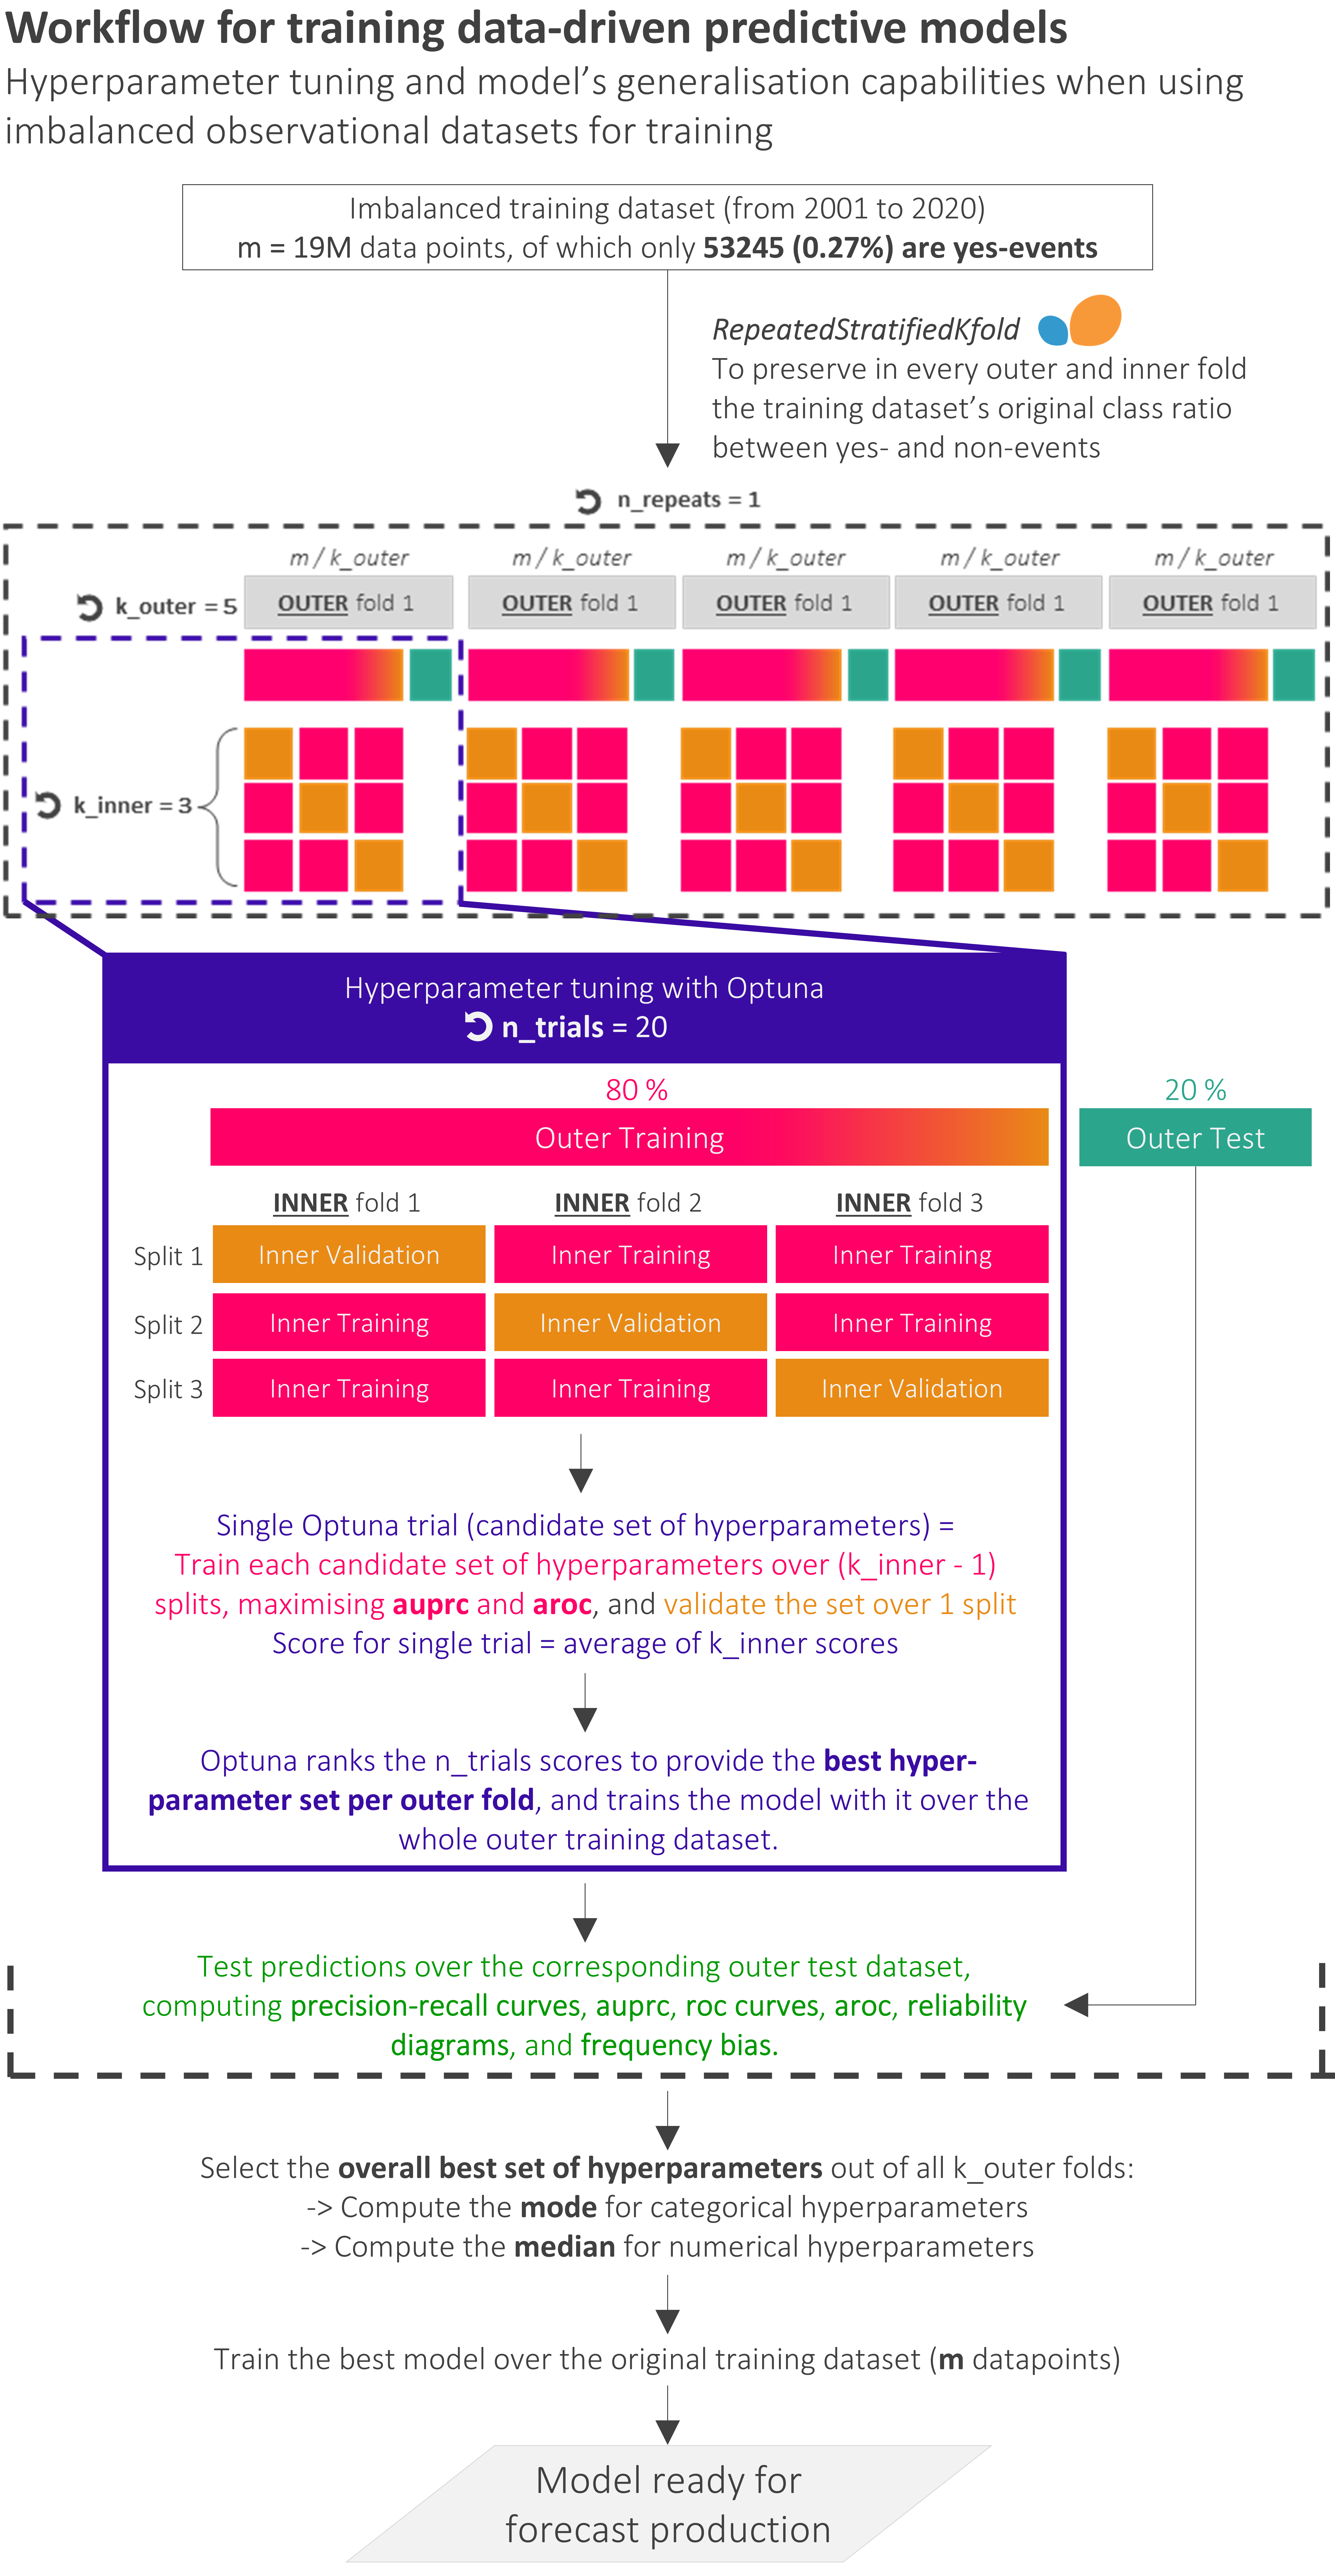
\includegraphics[scale=0.9]{chapter_06/figures/cv_optuna.png}
\caption{\textbf{Workflow for the repeated nested cross-validation.} The outer cross-validation loop utilises Scikit-Learn's "RepeatedStratifiedKFold" function to create k\_outer = 5 outer folds (grey blocks) across n\_repeats = 1 iterations. Each \textcolor{colourOuterFolds}{\textit{outer fold}} maintains the class distribution of the \textcolor{colourTraining}{\textit{training dataset}}, and it is split into an outer training dataset (80\%, blocks in shades of pink and orange) and an \textcolor{colourOuterTest}{\textit{outer test dataset}} (20\%). Within each outer fold, a Bayesian hyperparameter tuning is performed employing the Optuna library through an inner cross-validation procedure over n\_trial = 20 repetitions. Each trial evaluates candidate hyperparameters by training on \textcolor{colourInnerTraining}{\textit{inner training folds}} and validating on \textcolor{colourInnerValidation}{\textit{inner validation folds}}, with performance measured as the mean AUC-ROC or AUC-PR. The optimal hyperparameter set, identified by maximising the selected evaluation metric, is used to train the final model on the complete outer training subset. Model performance is assessed on the held-out \textcolor{colourOuterTest}{\textit{outer test fold}} using AUC-ROC and AUC-PR. The best-performing fold is retrained on the original \textcolor{colourTraining}{\textit{training dataset}} for operational deployment. Independent, more extensive verification of the data-driven predictions is performed using the \textcolor{colourTest}{\textit{verification dataset}}, considering the Precision-Recall curve and AUC-PR, the ROC curve and AUC-ROC, reliability diagrams, and frequency bias.}
\label{fig:cv_optuna}
\end{figure}

The outer cross-validation loop employed Repeated Stratified K-Fold cross-validation with 10 folds and 5 repetitions (n\_outer = 10, n\_repeats = 5), yielding 50 independent train-test splits. Each outer fold was processed independently to prevent information leakage.
Within each outer fold, an inner cross-validation loop was utilised for hyperparameter optimisation, implementing 5-fold cross-validation with 10 repetitions (n\_splits = 5, n\_repeats = 10). This configuration ensured robust hyperparameter selection based on 50 validation assessments per parameter configuration.


The methodology comprised nested cross-validation with Bayesian hyperparameter optimisation to ensure robust model selection and evaluation whilst mitigating overfitting in the context of imbalanced data. 















































% BUILT ROC CURVES: For the data-driven forecasts, where the forecast probability is provided by the model with continuous numbers between 0 and 1, the decision (probability) thresholds are defined by the user. In this thesis, a discretisation of 0.01 (equivalent to 1\%) and 0.001 (equivalent to 0.1\%) will be considered given the low frequency observed of flash flood events in the observational database. 




For hydro-meteorological, data-driven predictions, the verifying thresholds emerge directly from the machine learning algorithms that generated the predictions themselves, applying an optimisation that establishes the probability values that maximise the F1-score when converting a probabilistic prediction into a yes- or non-event. This data-driven threshold selection represents a departure from traditional approaches based, for example, on assumptions about the severity of the triggering events (as done for the rainfall-based forecasts). It instead allows the data-driven models themselves to identify optimal decision boundaries to convert the probabilistic forecasts into a yes or a non-event. As such, the thresholds will be defined based on the frequency of the yes-events in the observational datasets, delivering smaller verifying thresholds for rarer events. 


\subsection{Which verification metrics provide a comprehensive assessment of forecast quality?}

The verification framework employs a suite of metrics designed to evaluate different aspects of forecast performance, recognising that no single metric can fully characterise prediction quality for rare events like flash floods (pink area in Figure \ref{fig:workflow_verif_framework}). The selection of metrics addresses two primary forecast attributes: reliability and discrimination ability.

Reliability assessment examines whether predicted probabilities accurately reflect observed frequencies. The frequency bias provides an aggregate measure of systematic over- or under-prediction, whilst reliability diagrams offer detailed insights into calibration across the full probability spectrum. These metrics prove particularly valuable for understanding how well forecast systems capture the climatological frequency of flash floods, a fundamental requirement for risk-based decision making.

Discrimination ability quantifies the forecast system's capacity to distinguish between flood and non-flood situations. The Area Under the Receiver Operating Characteristic curve (AROC) provides a threshold-independent summary measure, whilst the full ROC curve reveals performance trade-offs at different probability thresholds. For rare event prediction, discrimination ability often represents the primary challenge, as models must identify subtle signals preceding infrequent occurrences.

The choice of probabilistic metrics reflects the inherent uncertainty in flash flood prediction and the need for risk-based decision frameworks in operational contexts. Deterministic metrics prove less suitable given the rarity of events and the importance of capturing forecast uncertainty. Detailed mathematical formulations and computational procedures are provided in the relevant analysis chapters.


\subsection{What training strategy ensures robust assessment of model performance when working with an extremely imbalanced dataset?}

The validation framework employs nested cross-validation with hyperparameter optimisation to provide unbiased performance estimates whilst maximising model performance. This approach addresses the risk of overfitting inherent in machine learning applications to imbalanced datasets.

The outer cross-validation loop uses stratified k-fold splitting to ensure representative class distributions in all data partitions. Within each outer fold, an inner optimisation loop identifies optimal hyperparameters using Bayesian optimisation via the Optuna framework. This nested structure prevents information leakage between hyperparameter selection and performance evaluation, providing realistic estimates of operational performance.
The choice of AROC as the optimisation metric during hyperparameter tuning reflects its suitability for imbalanced classification and alignment with the verification framework. Alternative metrics such as F1-score prove less suitable due to their dependence on classification thresholds and potential instability with extreme class imbalance.

Repeated evaluation across multiple cross-validation folds quantifies performance variability and identifies potential instabilities in model training. This comprehensive validation approach ensures that reported performance metrics reflect genuine predictive capability rather than fortunate data splits or overfitting to specific training samples. Implementation details and computational considerations are discussed in Chapter \ref{feasibility_PoFF}.


\subsection{How should flash flood observations be processed for grid-based verification?}

The transformation of point-based impact reports into gridded observational fields requires careful consideration of spatial and temporal aggregation methods. This study implements a systematic approach aligned with established severe weather verification methodologies \citep{Tsonevsky_2018, Pillosu_2024}.

Each flash flood report undergoes temporal aggregation to match the 24-hour accumulation periods of the forecast products, beginning at 00 UTC. This alignment ensures consistent comparison between observations and predictions whilst acknowledging that flash floods may occur at any time within the accumulation window. The choice of 24-hour periods balances the need for sufficient temporal resolution with the practical constraints of forecast product availability and the typical duration of flash flood events.

Spatial assignment of reports to the ERA5 grid (approximately 31 km resolution) employs a nearest-neighbour approach for point reports and polygon inclusion for events with spatial extent. Given the relatively coarse resolution of ERA5 grid boxes compared to typical flash flood scales, additional spatial expansion techniques commonly used in convective-scale verification prove unnecessary. The resulting gridded fields preserve information about event frequency within each grid box, enabling more nuanced verification than binary occurrence fields.
This processing approach addresses the fundamental challenge of scale mismatch between localised flash flood events and gridded forecast products. The methodology provides a reproducible framework applicable to other grid resolutions and accumulation periods, with detailed implementation provided in chapter \ref{flash_flood_focused_verification_framework}.



%%%%%%%%%%%%%%%%%
\section{Results}
\label{data_driven_flash_floods_short_medium_range_results}


\subsection{Model training}

\subsubsection{Training methodology}

The development of the data-driven predictions of areas at risk of flash floods employed a systematic training approach designed to optimise predictive performance whilst ensuring generalisability due to the severe imbalance problem in the training dataset. 

The model architectures comprised decision-tree-based algorithms such as random forest and gradient boosting (XGBoost and CatBoost), and a feed-forward neural network. We considered 7 input features such as the probability of exceeding a certain rainfall return period, the maximum probability of exceeding a certain rainfall return period in the adjacent grid-boxes within a radius, the antecedent soil moisture, the steepness of the orography, and the vegetation coverage. 

The training dataset comprises 53,245 yes-events over 19,746,990 grid-boxes (0.27\% of yes-events), spanning the years between 2001 to 2020. 

To ensure a robust model evaluation and prevent overfitting, a nested cross-validation strategy was implemented, employing 5-fold cross-validation for the outer loop and 3-fold for hyperparameter optimisation in the inner loop. 

The input feature set underwent normalisation for the neural network, calculated independently for each training fold to prevent data leakage.

No missing values strategies was applied to the dataset as there not were any by design.


\subsubsection{Hyperparameter optimisation}

Hyperparameter selection employed Optuna (version 4.3.0), a state-of-the-art hyperparameter optimisation framework utilising Tree-structured Parzen Estimator (TPE) sampling. This Bayesian optimisation approach was integrated within the inner loop of the nested k-fold cross-validation procedure, ensuring unbiased performance estimates whilst identifying optimal hyperparameter configurations.

For each outer fold, an independent Optuna study was initiated with 20 trials, allowing the algorithm to explore the hyperparameter space. The objective function maximised the mean AROC across the inner k-fold cross-validation splits, with early pruning implemented via Optuna's MedianPruner to terminate unpromising trials and reduce computational overhead.

Figure \ref{fig:optuna_optimasation_convergence} illustrates the optimisation history for the five outer folds, demonstrating the TPE algorithm's efficiency in identifying high-performing configurations from the first iteration. The solid coloured lines track the trails with the "best value" for the objective (i.e. maximising AROC). The best trial appears to be in all cases trial n. 0, until convergence towards optimal values typically occurred within 10 and 15 trials. Optuna run the full set of 20 trials for all outer loops as shown in Figure \ref{fig:optuna_optimasation_convergence}.

\begin{figure}[htbp]
\centering
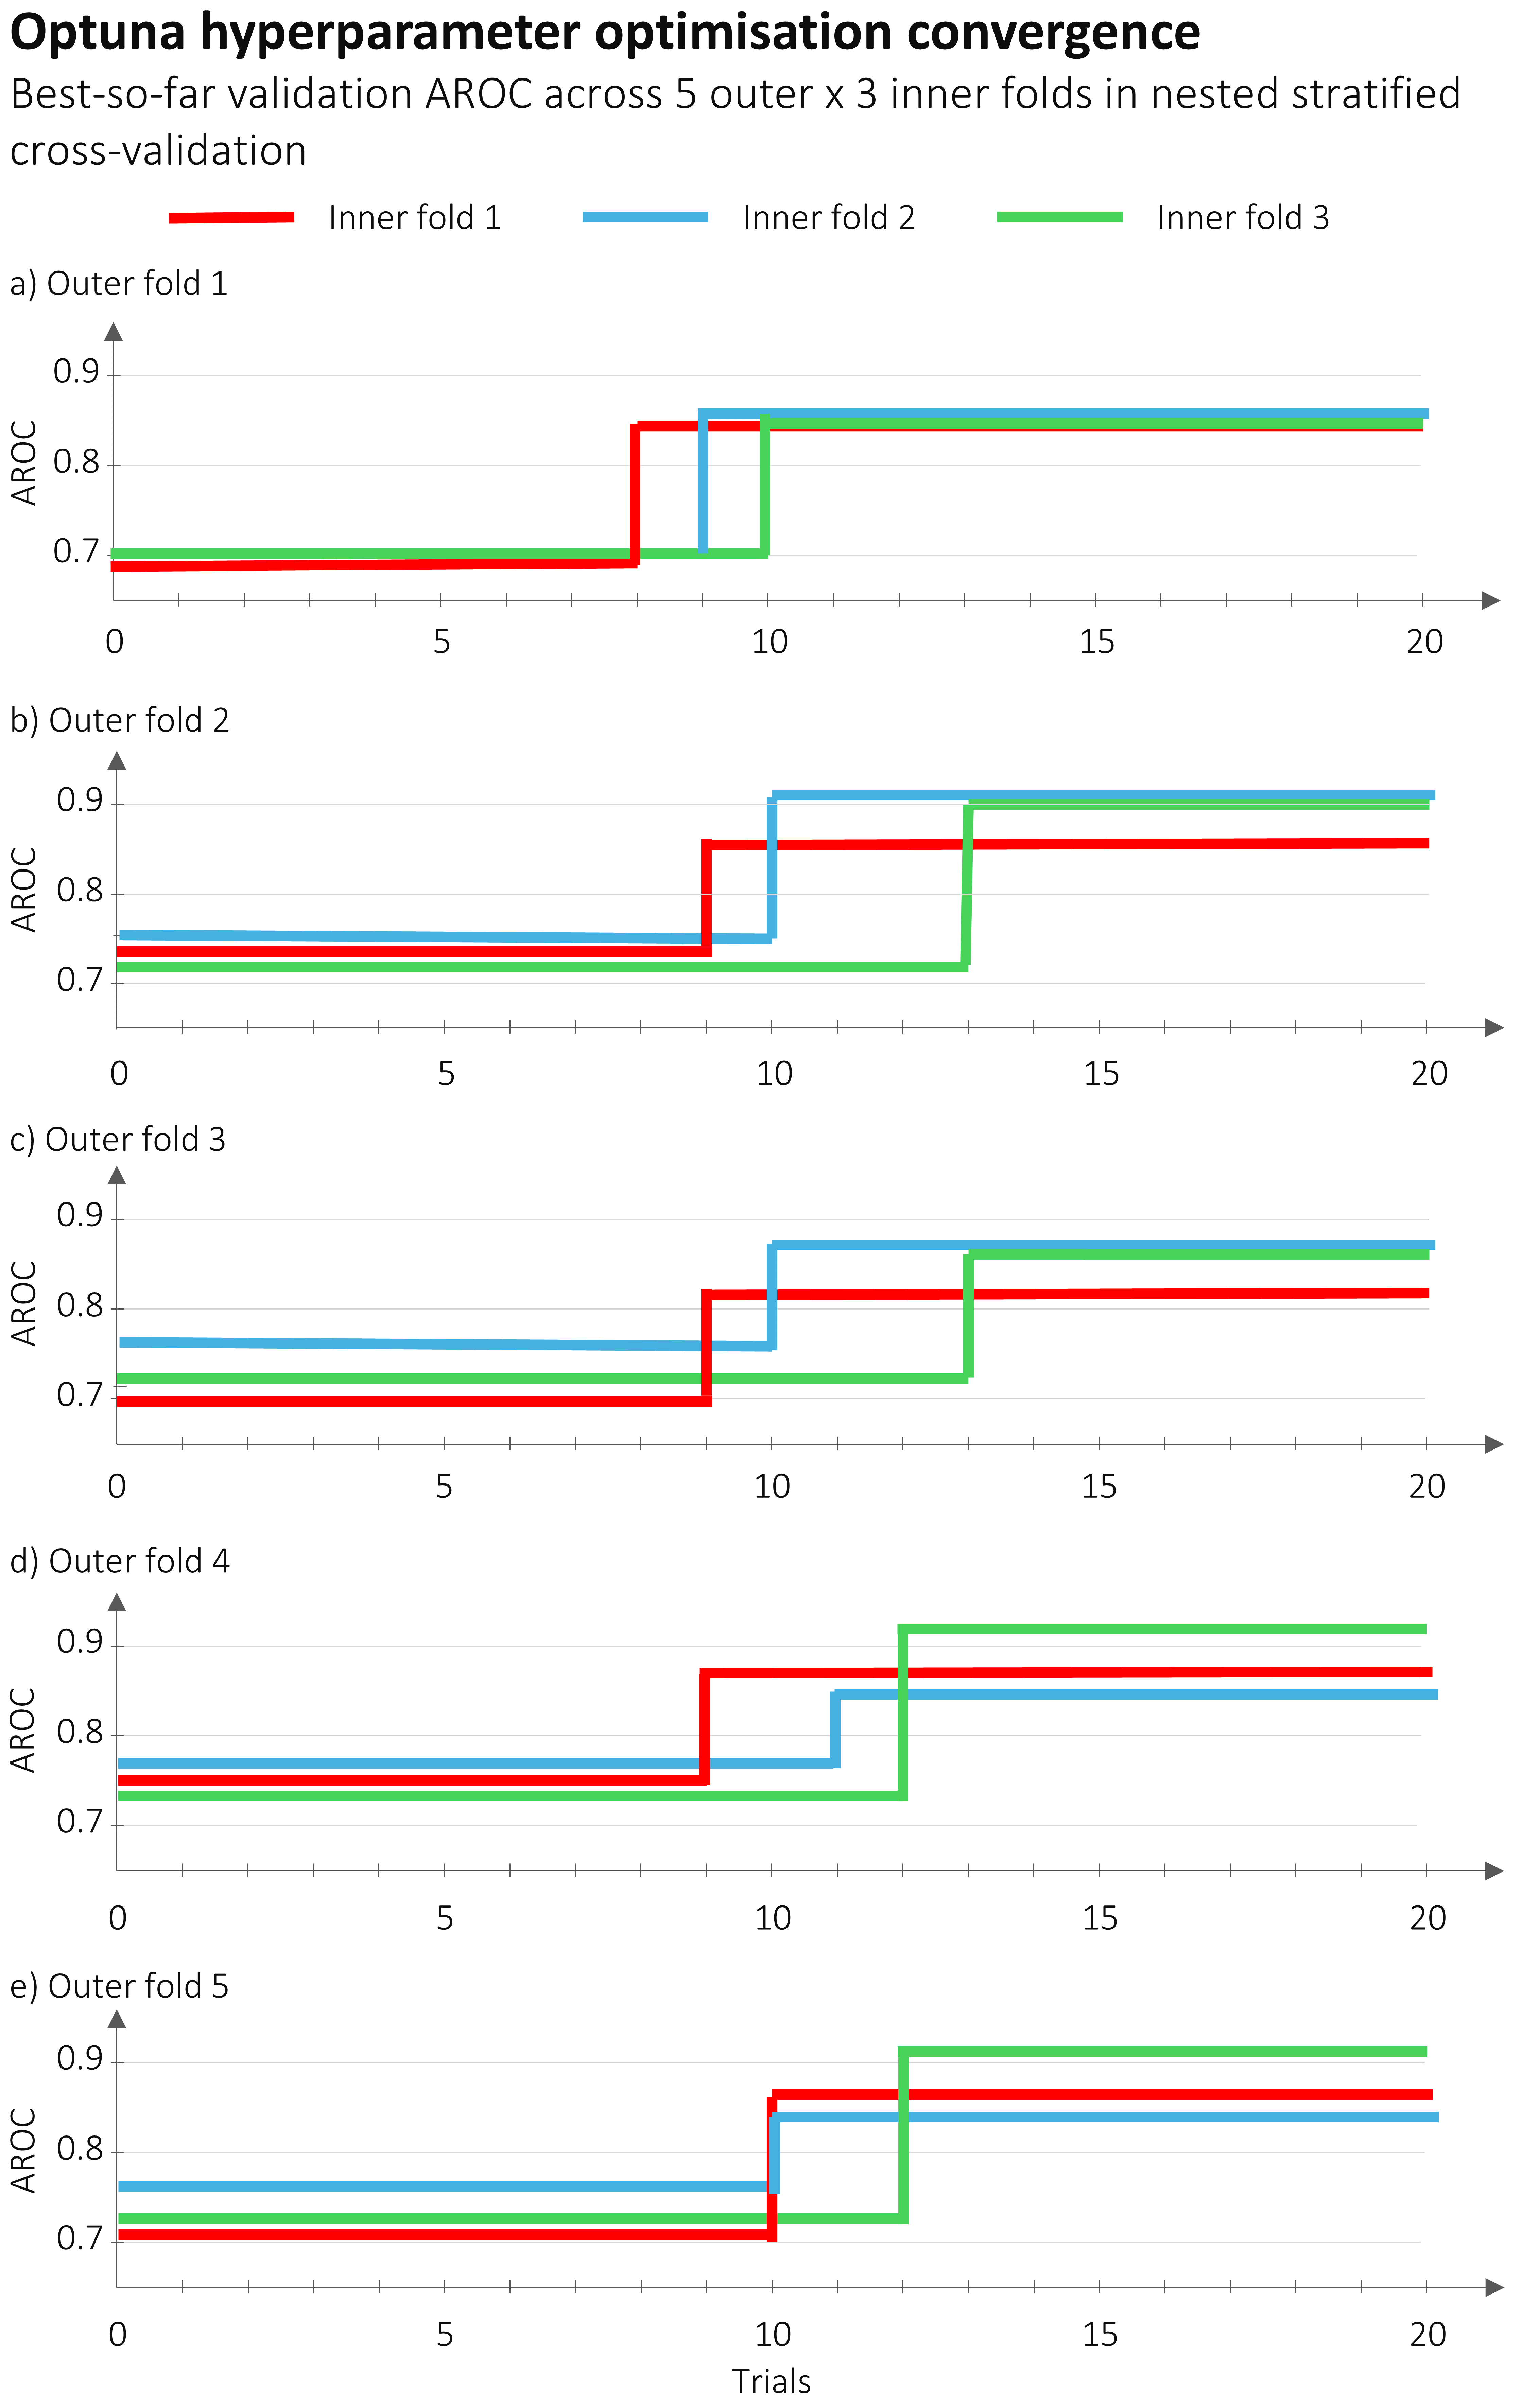
\includegraphics[width=\textwidth]{optuna_optimasation_convergence.png}
\caption{\textbf{Convergence of Optuna hyperparameter optimisation during nested stratified 5 × 3 cross-validation} Panels (a) to (e) correspond to the outer folds. Within each panel, the three coloured staircase lines show the running best validation area under ROC curve returned from the three inner folds over the 20 trials of the hyper-parameter search. A sharp improvement is typically found between trials \sim8–13, after which the curves flatten, indicating that the optimiser converges.}
\label{fig:optuna_optimasation_convergence}
\end{figure}

The optimisation procedure yielded distinct optimal configurations for each outer fold, reflecting data heterogeneity across splits. Table 4.1 summarises the selected hyperparameter values and corresponding validation performance for each fold, demonstrating reasonable consistency in optimal values despite fold-specific variations.


\subsubsection{Training progression and convergence}

Figure \ref{fig:hydro_based_ff_cross_validation_optuna_overall_scores} presents the performance stability across the five outer folds for all evaluated models for overall scores such as AROC, recall and F1-score. In all models, the AROC values exhibited remarkable consistency across folds, with the gradient boosting implementations (XGBoost and LightGBM) maintaining values between 0.84 and 0.86 throughout. The random forest variants demonstrated slightly lower (AROC between 0.81 and 0.83) but equally stable performance. The CatBoost implementation of gradient boosting showed the lowest performance (AROC \sim0.8) of all decision-tree-based models, and the feed-forward neural network showed the lowest performance with AROC values between 0.78 and 0.8. While XGBoost remains the best model based on the recall and the F1-score, the model ranking based on these metrics shows higher variability depending on the outer fold. The small variations in the scores' absolute values suggest that such ranking differences are primarily attributable to class imbalance sensitivity to rare positive instances rather than training instability. 

\begin{figure}[htbp]
\centering
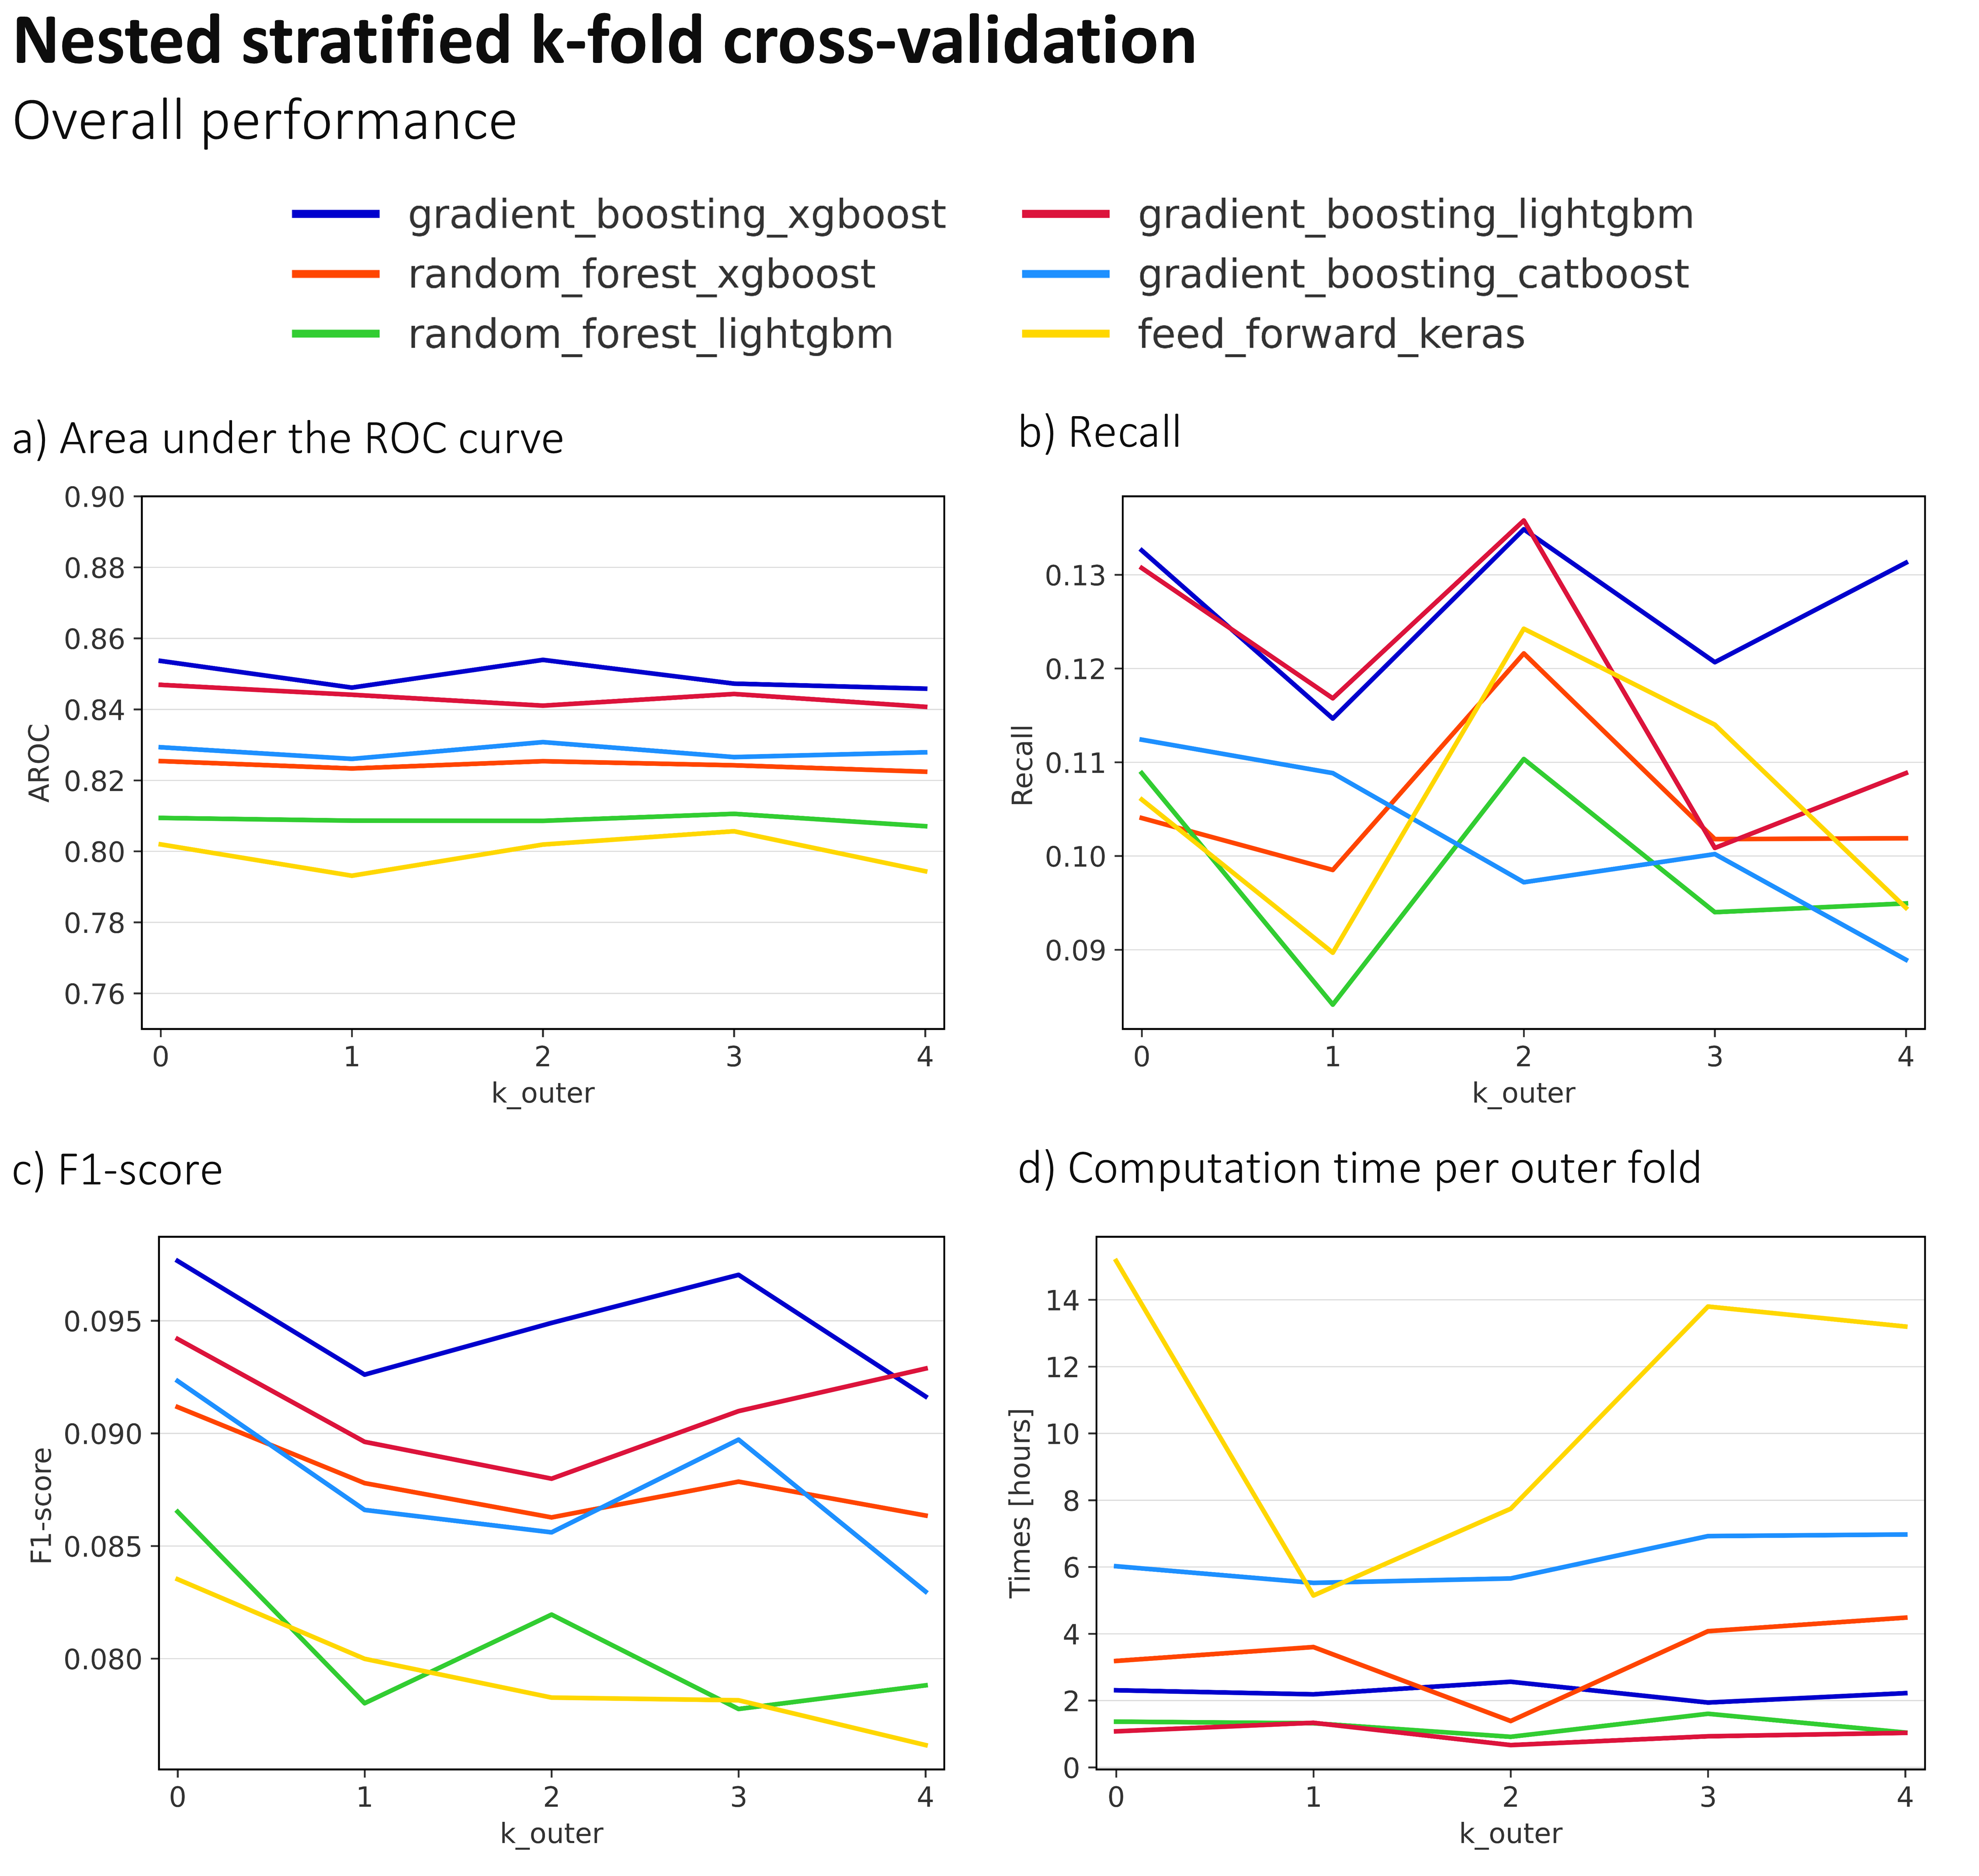
\includegraphics[width=\textwidth]{hydro_based_ff_cross_validation_optuna_overall_scores.png}
\caption{\textbf{Overall scores to estimate the model performance during the nested stratified k-fold cross validation.} Panels (a) to (d) show the values for, respectively, the area under the ROC curve, recall, F1-score, and training + hyperparameter optimisation time per outer fold. The solid colour lines represent the different models: gradient boosting - XGBoost implementation - in blue, gradient boosting - LightGBM implementation - in red, gradient boosting - CatBoost implementation - in cyan, random forest - XGBoost implementation - in orange, random forest - LightGBM implementation - in green, and feed forward neural network in yellow.}
\label{fig:hydro_based_ff_cross_validation_optuna_overall_scores}
\end{figure}

The ROC curves and the reliability diagrams (Figure \ref{fig:hydro_based_ff_cross_validation_optuna_breakdown_scores}) further illustrate the convergence quality by examining the discrimination ability and the reliability consistency across folds. Overall, the gradient boosting models (XGBoost - first column, LightGBM - second column, and Catboost - third column) show the best ROC curves and reliability diagrams, compared to the random forest implementations and the neural network, with high consistency across the outer folds. However, XGBoost shows again the best performance of all with the "optimal operating point" in the ROC curves being at a hit rate around \sim0.8 and a false alarm rate around only \sim0.3, and predicted probabilities in the reliability diagram closely aligning with the observed frequencies across most probability ranges (up to 25\% and reaching 50\% in the outer fold 1). While the other models show similar ROC curves, although with optimal operating points around hit rate of \sim0.7 for the decision-tree-based models and \sim0.6 for the neural network, the reliability diagrams for this models show a tendency to overestimate (i.e. the diagrams lie below the diagonal) from probabilities exceeding 10\% for the LightGBM and CatBoost implementations of the gradient boosting, and for almost all probability ranges in the random forest implementation of LightGBM. The XGBoost implementation of the random forest model shows a similar reliability to the XGBoost implementation of the gradient boosting, but the discrimination ability of the latter model is superior (better ROC curves over all outer folds). This suggests that \textit{gradient boosting} performs overall better than random forests when using imbalanced training datasets.

Special attention should be given to the neural network as it shows an overall good reliability (i.e. the predicted probabilities are close to the diagonal) but,  compared to the decision-tree-based models, the neural network does not provide high predicted probabilities, as they do not exceed 25\% (it reaches 50\% in only one outer fold). This behaviour suggests that the neural network demonstrates a conservative but reliable forecasting behaviour. While the neural network restraint in issuing high-probability forecasts might reflect a better uncertainty quantification and more reliable risk communication for operational deployment, the XGBoost implementation of the gradient boosting shows that predicted probabilities higher than 25\% can also be reliable between 30\% and 50\%. This restricted probability range in the neural network predictions presents operational challenges, as the model fails to differentiate between moderate and high-risk events, as shown by the lower discrimination ability of the neural network compared to XGBoost.. The inability to forecast probabilities above 25\% effectively compresses the decision space for emergency managers, who require clearer discrimination between events warranting different levels of response. Whilst a forecast of 25\% probability might trigger initial preparedness measures, operational protocols often stipulate enhanced response actions at higher probability thresholds (e.g., 40\%, 60\%). The neural network's truncated probability distribution therefore limits its utility in supporting graduated response strategies, potentially resulting in either insufficient preparation for genuinely high-risk events or uniform treatment of situations with materially different risk levels. This operational limitation suggests that, despite its superior calibration at lower probabilities, the neural network may be less suitable than the gradient boosting approaches for applications requiring nuanced risk stratification.

\begin{figure}[htbp]
\centering
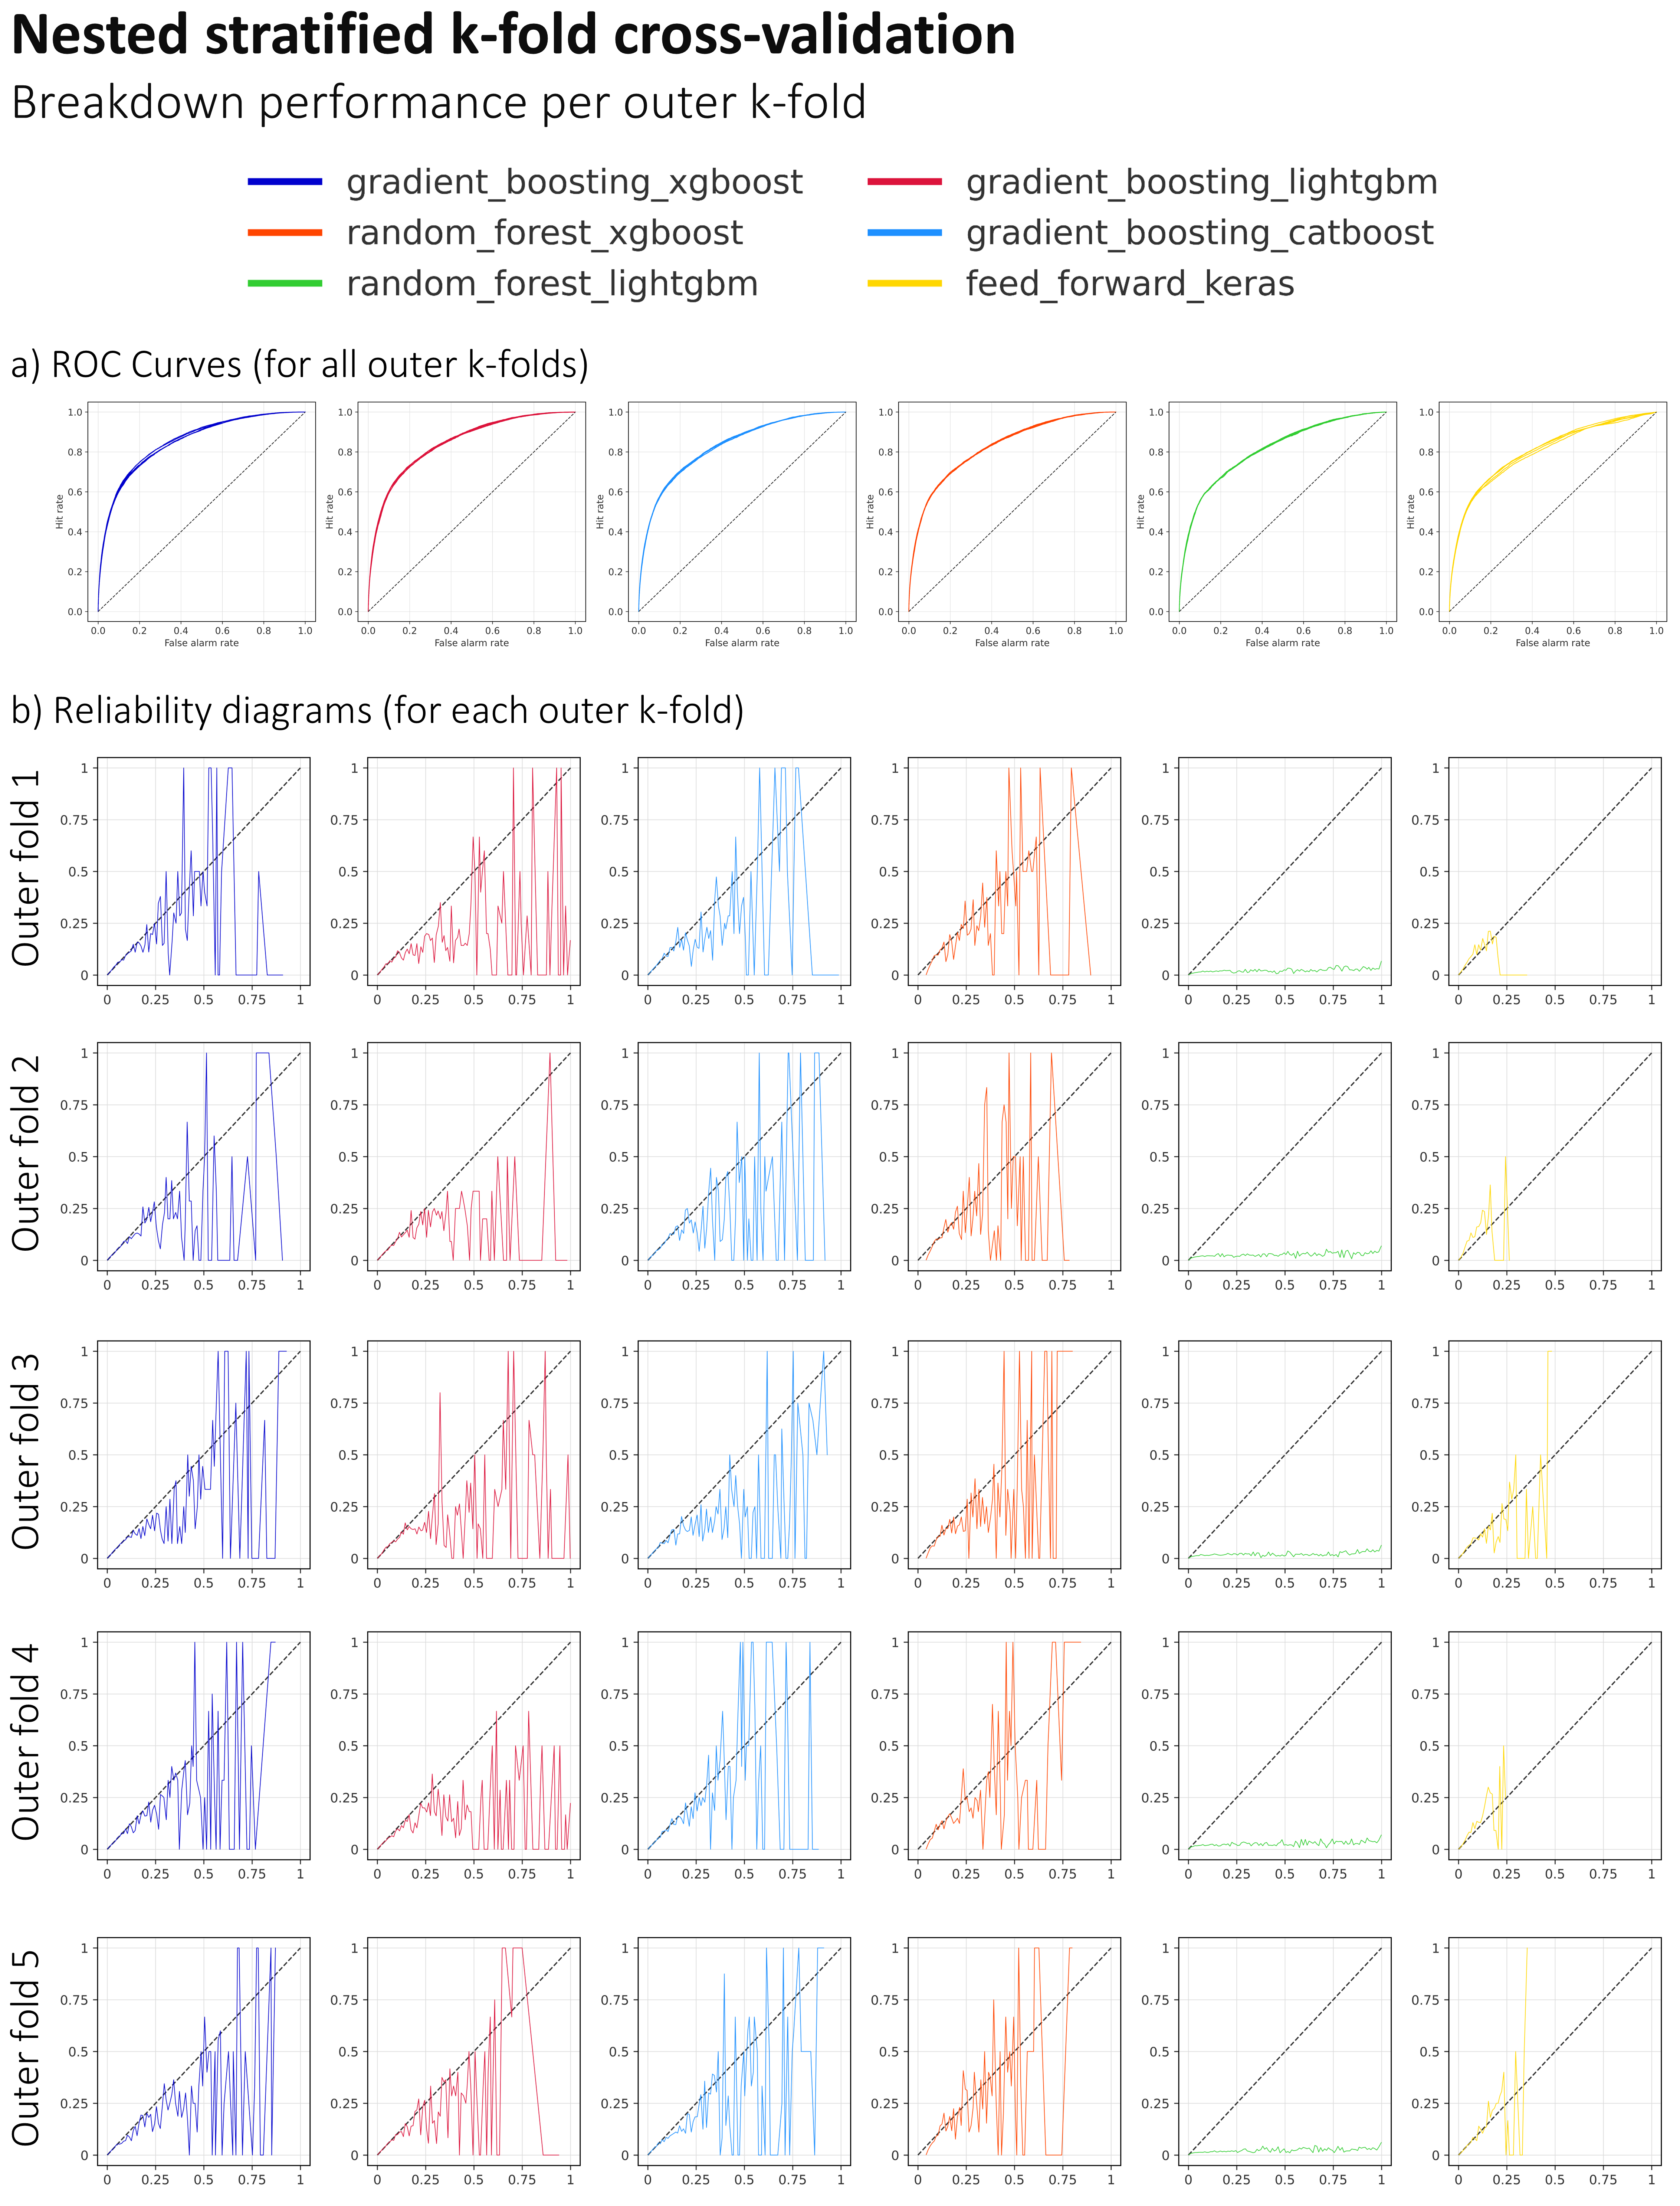
\includegraphics[width=\textwidth]{hydro_based_ff_cross_validation_optuna_breakdown_scores.png}
\caption{\textbf{Breakdown scores to estimate the model performance during the nested stratified k-fold cross validation.} Figures in panel (a) show the ROC curves for all the outer loops for gradient boosting - XGBoost implementation - in blue, gradient boosting - LightGBM implementation - in red, gradient boosting - CatBoost implementation - in cyan, random forest - XGBoost implementation - in orange, random forest - LightGBM implementation - in green, and feed forward neural network in yellow. Figures in panel (b) show the reliability diagrams for each outer loop (rows) and each model (columns).}
\label{fig:hydro_based_ff_cross_validation_optuna_breakdown_scores}
\end{figure}

In conclusion, the stability of model rankings across folds provided additional evidence of training convergence. The gradient boosting XGBoost consistently achieved the highest discrimination performance, followed closely by LightGBM, whilst the random forest implementations and neural networks occupied lower performance tiers. This consistent hierarchy across independent training runs confirms that the observed performance differences reflect genuine algorithmic characteristics rather than training artefacts or convergence failures.


\subsubsection{Final model selection}

Based on the performance metrics across all outer cross-validation folds (Figure \ref{fig:hydro_based_ff_cross_validation_optuna_overall_scores} and Figure \ref{fig:hydro_based_ff_cross_validation_optuna_breakdown_scores}, the model considered in this thesis to create the predictions of areas at risk of flash floods is the XGBoost implementation of the gradient boosting.

To establish the final model configuration for deployment (Table \ref{}), the hyperparameter values were aggregated across the outer folds using the \textit{median for continuous parameters} and the \textit{mode for categorical parameters}. This ensemble approach provided robustness against fold-specific peculiarities whilst maintaining near-optimal performance. 

\begin{table}[htbp]
\centering
\captionof{table}{\textbf{Final (optimal) configuration for the XGBoost implementation of the gradient boosting}. Values of the hyperparameters.}
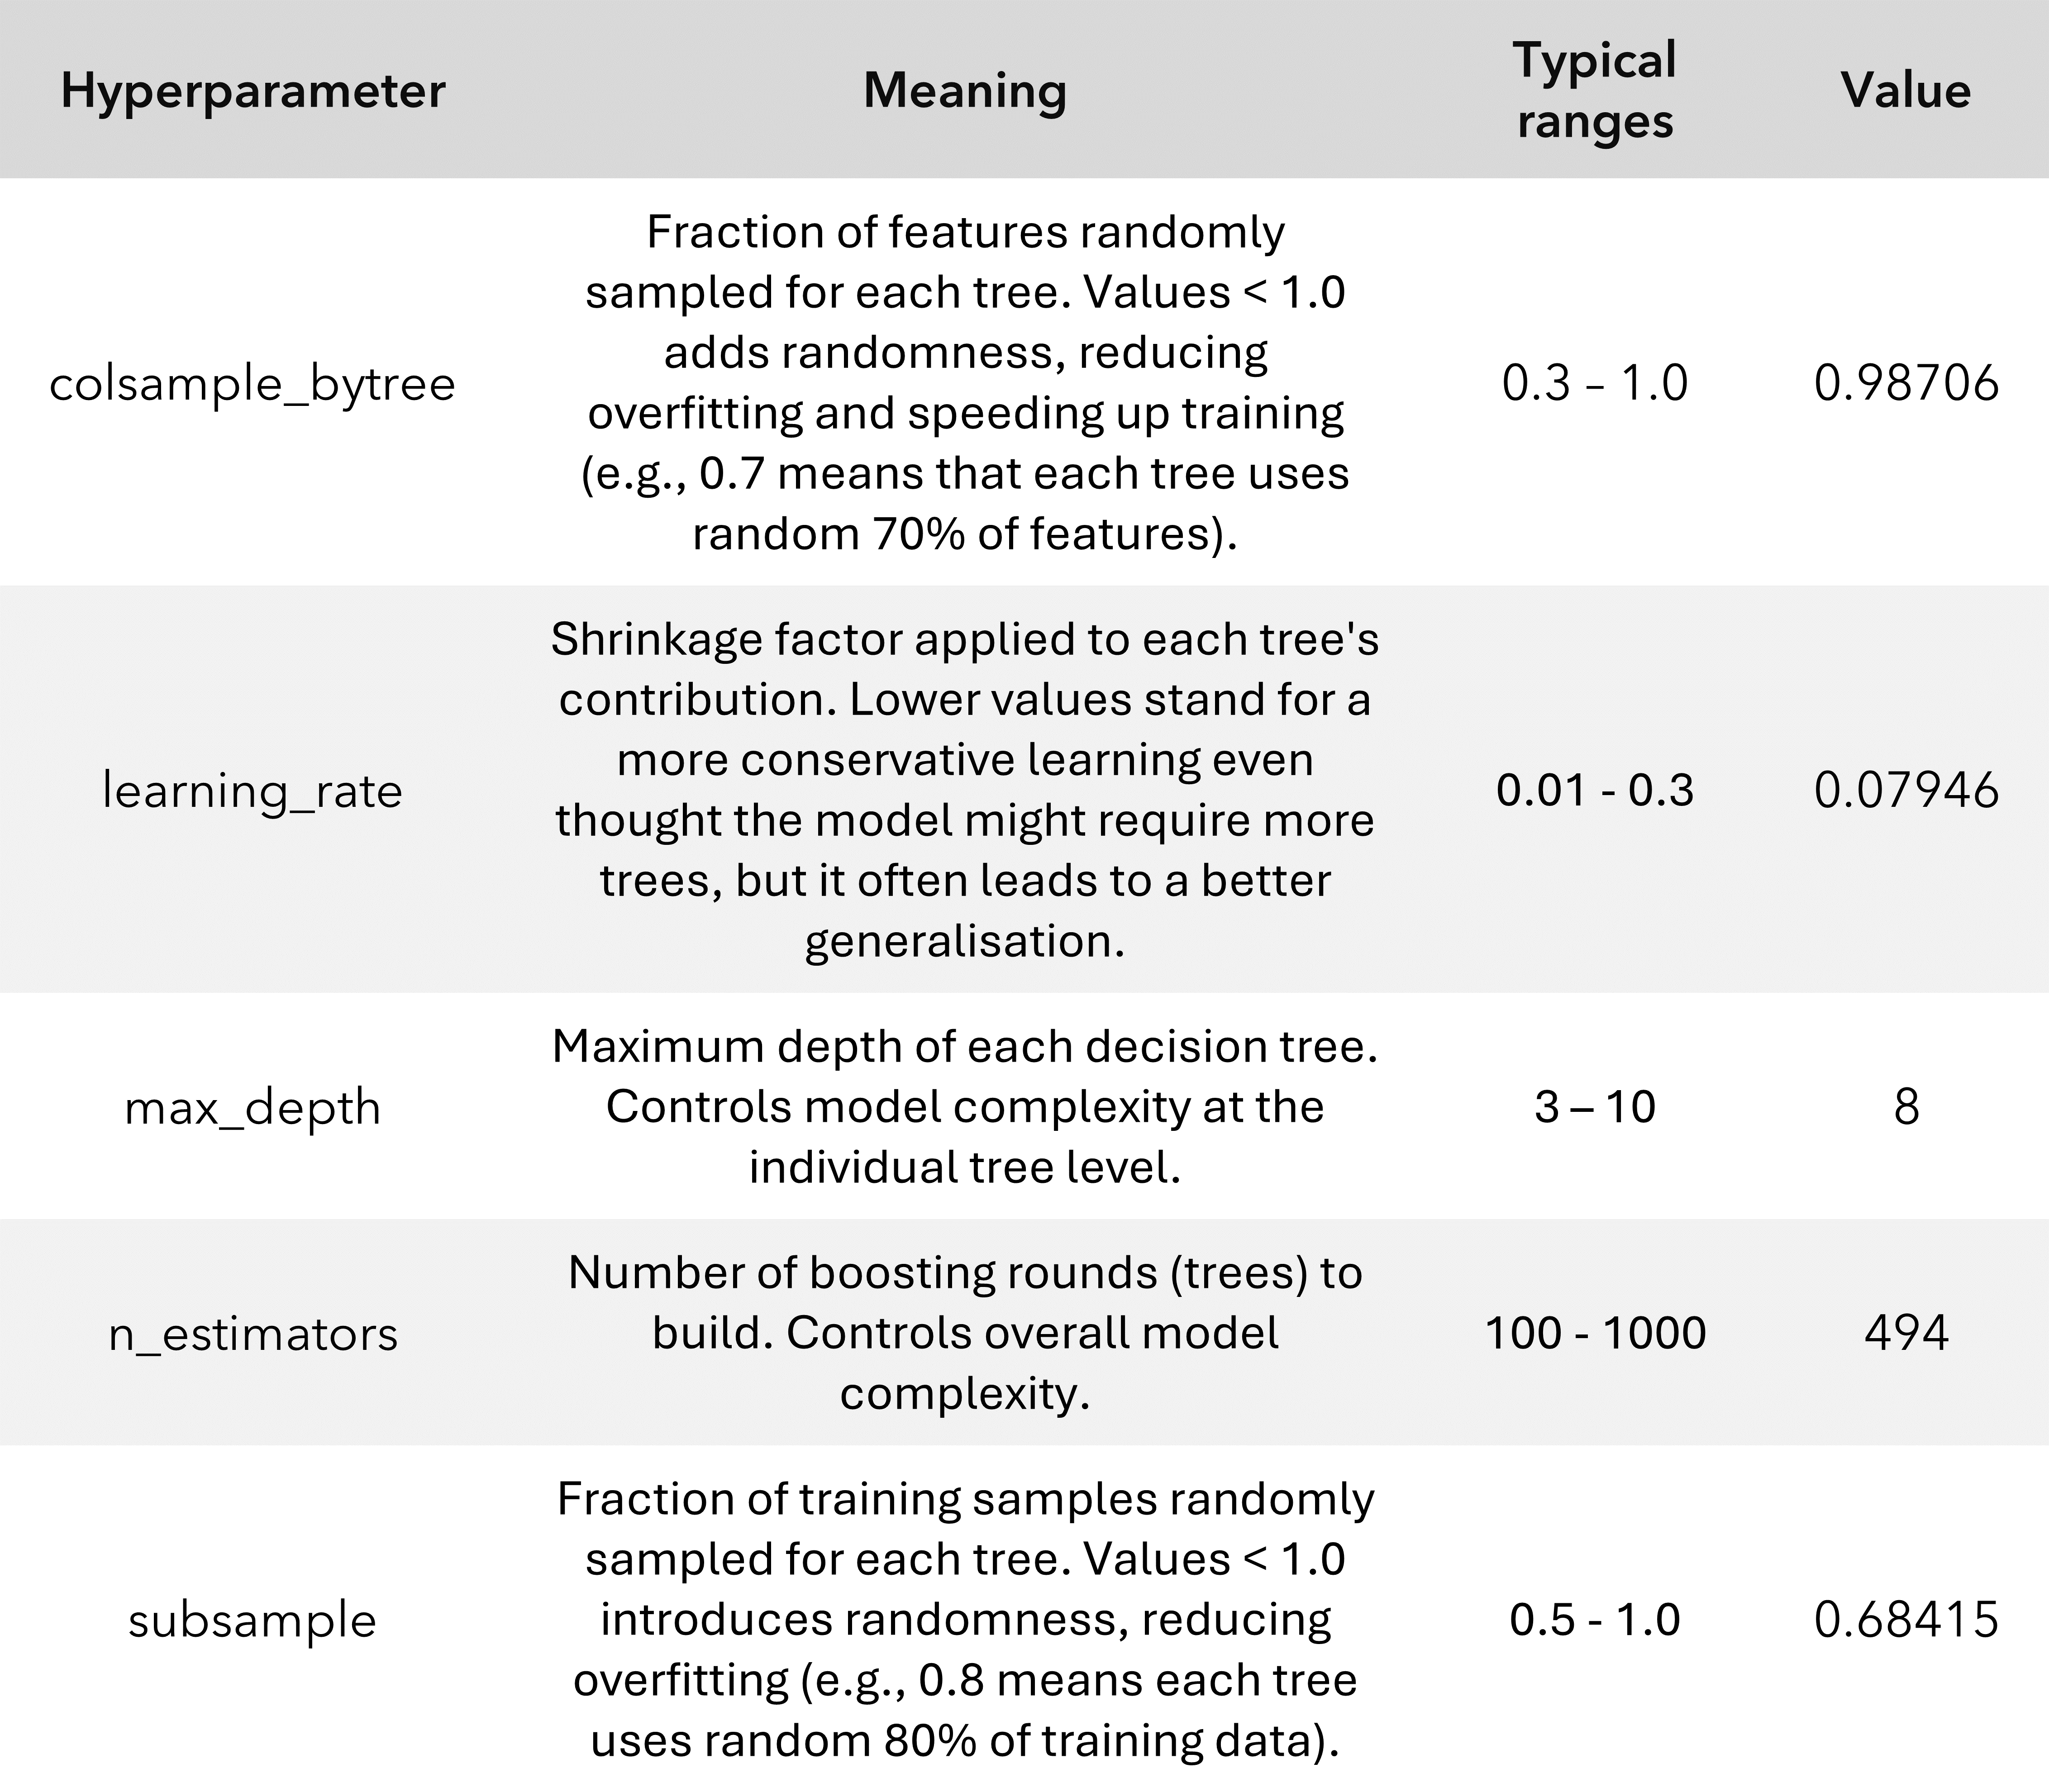
\includegraphics[width=\textwidth]{xgboost_final_configuration.png}
\label{table:xgboost_final_configuration}
\end{table}

The optimal XGBoost configuration identified through hyperparameter optimisation represents a moderately complex ensemble with careful regularisation to prevent overfitting. The model comprises 494 gradient boosted trees, each limited to a maximum depth of 8 levels, striking a balance between capturing non-linear patterns and maintaining interpretability. The learning rate of 0.07946 indicates a relatively conservative training approach, where each successive tree contributes only 7.9\% of its predictions to the ensemble, requiring the full complement of trees to achieve optimal performance whilst avoiding overshooting the loss function minima. This configuration employs substantial stochastic regularisation through both row and column subsampling: each tree is trained on a random 68.4\% of the training instances (subsample = 0.684) and utilises 98.7\% of available features (colsample\_bytree = 0.987). The high colsample\_bytree value (near 1.0) suggests that feature subsampling provides minimal regularisation benefit for this dataset, indicating that most predictors contribute meaningful information for flash flood prediction. Conversely, the moderate row subsampling (subsample = 0.68415) introduces beneficial stochasticity, helping the model generalise beyond the training data whilst maintaining sufficient data for reliable tree construction.

This configuration reflects a model that prioritises stability and generalisation over aggressive fitting, appropriate for the high-stakes nature of flash flood forecasting, where false alarms and missed events carry significant consequences. The parameter combination suggests the optimisation process favoured a large ensemble of moderately deep trees with conservative learning dynamics over a smaller set of more complex trees, likely improving the model's robustness to variations in hydro-meteorological conditions.

\subsubsection{Computation requirements}



\subsection{Assessment of short- and long-range data-driven hydro-meteorological predictions of areas at risk of flash floods}

\subsubsection{Overall verification scores}

Figure \ref{fig:hydro_based_ff_verif_overall_scores} presents the results of the objective verification analysis carried out on the hydro-meteorological, data-driven predictions of areas at risk of flash floods. It shows distinct performance characteristics between the short-range forecasts (also known as reanalysis) and the long-range forecasts (up to t +120, day 5). It is worth noticing that day 1 forecasts (t+24) have a very similar value compared to those for day 0 (short-range) forecasts, in all verification scores. 

The area under the ROC curve (Figure \ref{fig:hydro_based_ff_verif_overall_scores}a) shows forecasts with strong discrimination ability, maintaining values above 0.75 across all lead times. The short-range forecast (lead time 0) and day 1 forecasts achieve the highest discrimination performance with an AROC of approximately 0.83, indicating excellent ability to distinguish between flash flood and non-flash flood events. As lead time increases, the AROC exhibits a gradual linear decline, reaching \sim0.77 at day 5 forecasts (\sim7\% reduction in discrimination ability from day 0). Such a small reduction, especially compared to the rainfall-based forecasts, represents a modest degradation considering the extended forecast range, suggesting that the model maintains substantial predictive skill even at longer lead times.

The frequency bias (Figure \ref{fig:hydro_based_ff_verif_overall_scores}b) reveals a dramatic shift in forecast behaviour between short-range and long-range predictions. The day 1 forecasts show nearly identical frequency bias compared to day 0 (short-range) forecasts, i.e, \sim15. From day 2 forecasts, the frequency bias starts increasing, reaching a frequency bias that doubles the one at day 1 (\sim 31) at day 4. Comparing these results to the rainfall-based forecasts, where the frequency bias remains mostly constant over the different lead times, it would not be reasonable to think that the degradation of the frequency bias in the hydro-meteorological, data-driven forecasts are mainly due to variations in skill of the soil moisture with lead time, as the other parameters adopted in the data-driven model (orography and vegetation cover, are either static or climatological).

The recall (Figure \ref{fig:hydro_based_ff_verif_overall_scores}c) and F1-score (Figure \ref{fig:hydro_based_ff_verif_overall_scores}d) show a similar pattern. The day 1 forecasts show a slightly higher value compared to the one at day 0 (\sim 0.11 for recall and 0.08 for F1-score). From day 2, both scores half around day 5. This means that, according to both metrics, the model's ability to detect true positives deteriorates significantly beyond day 2, with the 5-day forecast detecting \sim half the events identified by the short-range forecast or the day 1 forecasts.

These verification metrics collectively indicate that the data-driven approach performs optimally at 0-1 day lead times, with acceptable performance extending to day 2. Beyond this threshold, whilst discrimination ability (AROC) remains reasonable, the operational utility diminishes substantially due to excessive false alarm rates and reduced detection capability, suggesting to further adjust the lead-time-dependent probability thresholds or alternative modelling strategies for extended-range flash flood forecasting.

\begin{figure}[htbp]
\centering
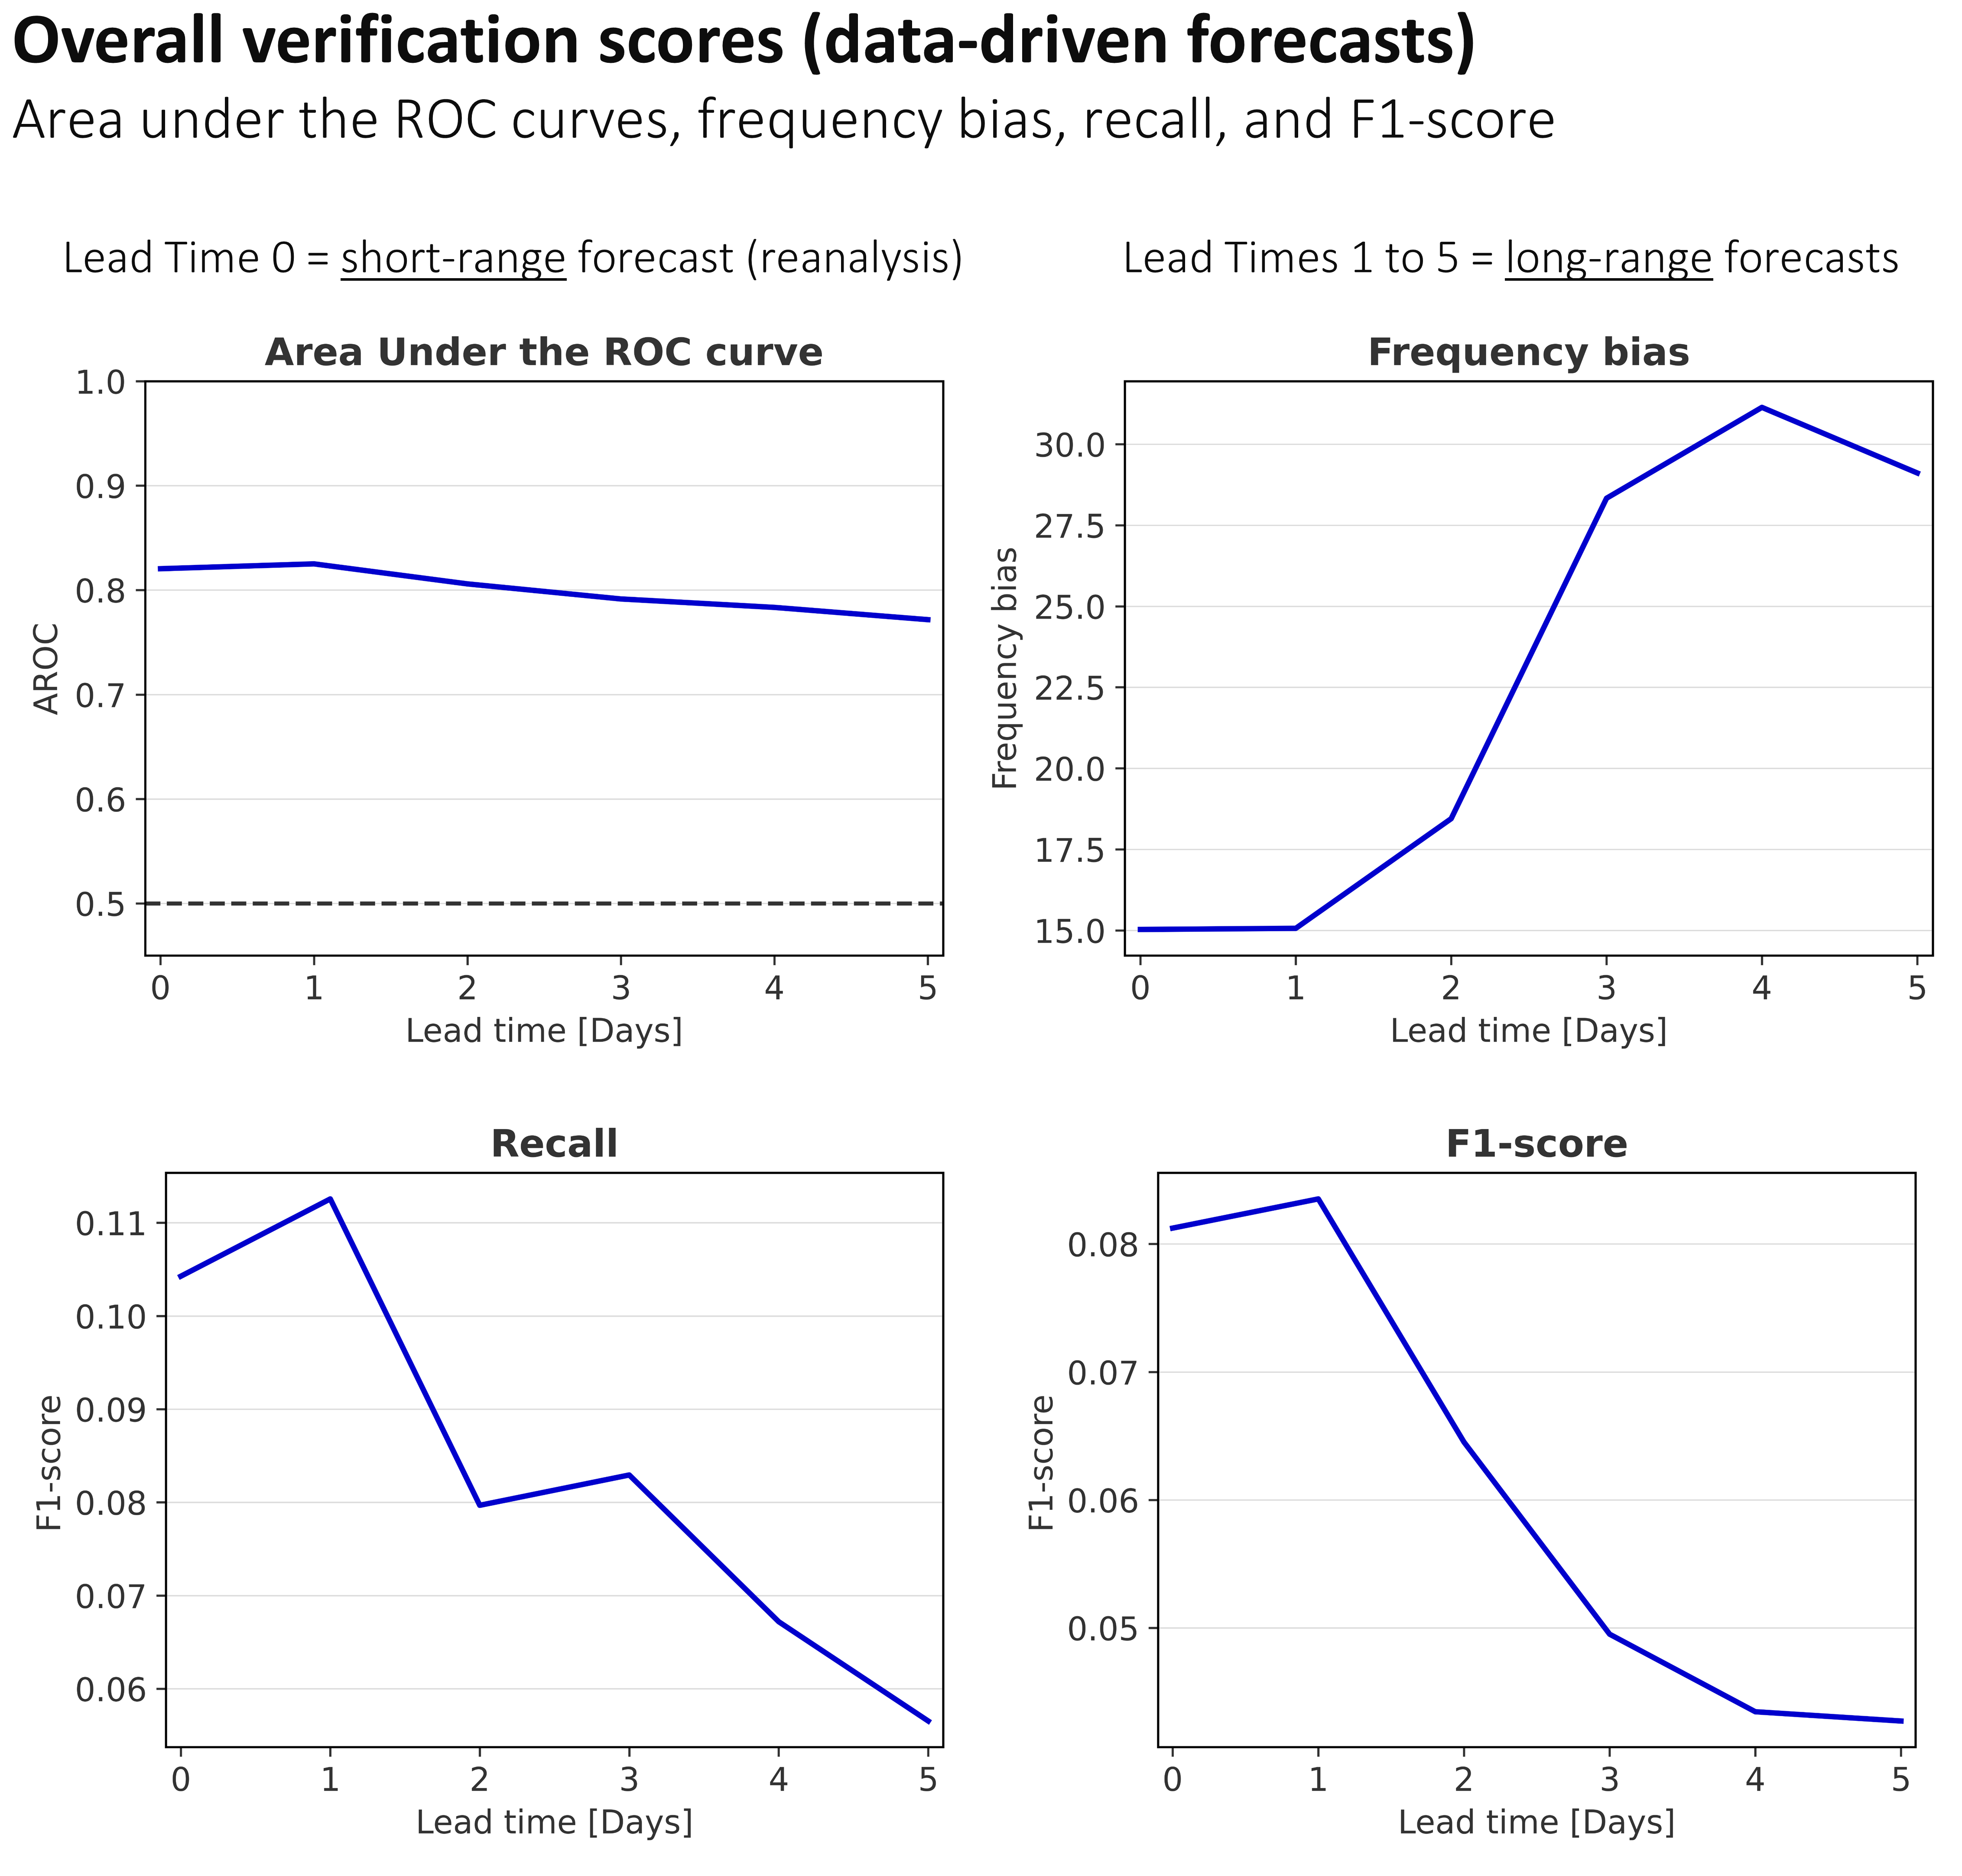
\includegraphics[width=\textwidth]{hydro_based_ff_verif_overall_scores.png}
\caption{\textbf{Overall verification scores for data-driven, hydro-meteorological forecasts.} Panel (a) shows the Area under the ROC curve for the short-range forecasts (i.e., reanalysis, lead time = 0), and the long-range forecasts (lead time = 1 - t+24, lead time = 2 - t+48, lead time = 3 - t+72, lead time = 4, t+96, lead time = 5, t+120). Panels (b) to (c) show, respectively, the frequency bias, the recall, and the F1-score.}
\label{fig:hydro_based_ff_verif_overall_scores}
\end{figure}

\subsubsection{Breakdown verification scores}

As seen in the overall verification scores, also the ROC curve for a day 1 (Figure \ref{fig:hydro_based_ff_verif_breakdown_scores_roc}, dashed line) forecast is nearly identical (almost perfect overlap) with day 0 forecasts (\ref{fig:hydro_based_ff_verif_breakdown_scores_roc}, solid and thicker line). Then, there is a small and gradual worsening of the ROC for longer-range forecasts observed by the flattening of the ROC curves towards the diagram's diagonal. Such flattening means that for a similar hit rate, the false alarms increase slightly, around 0.1.

\begin{figure}[htbp]
\centering
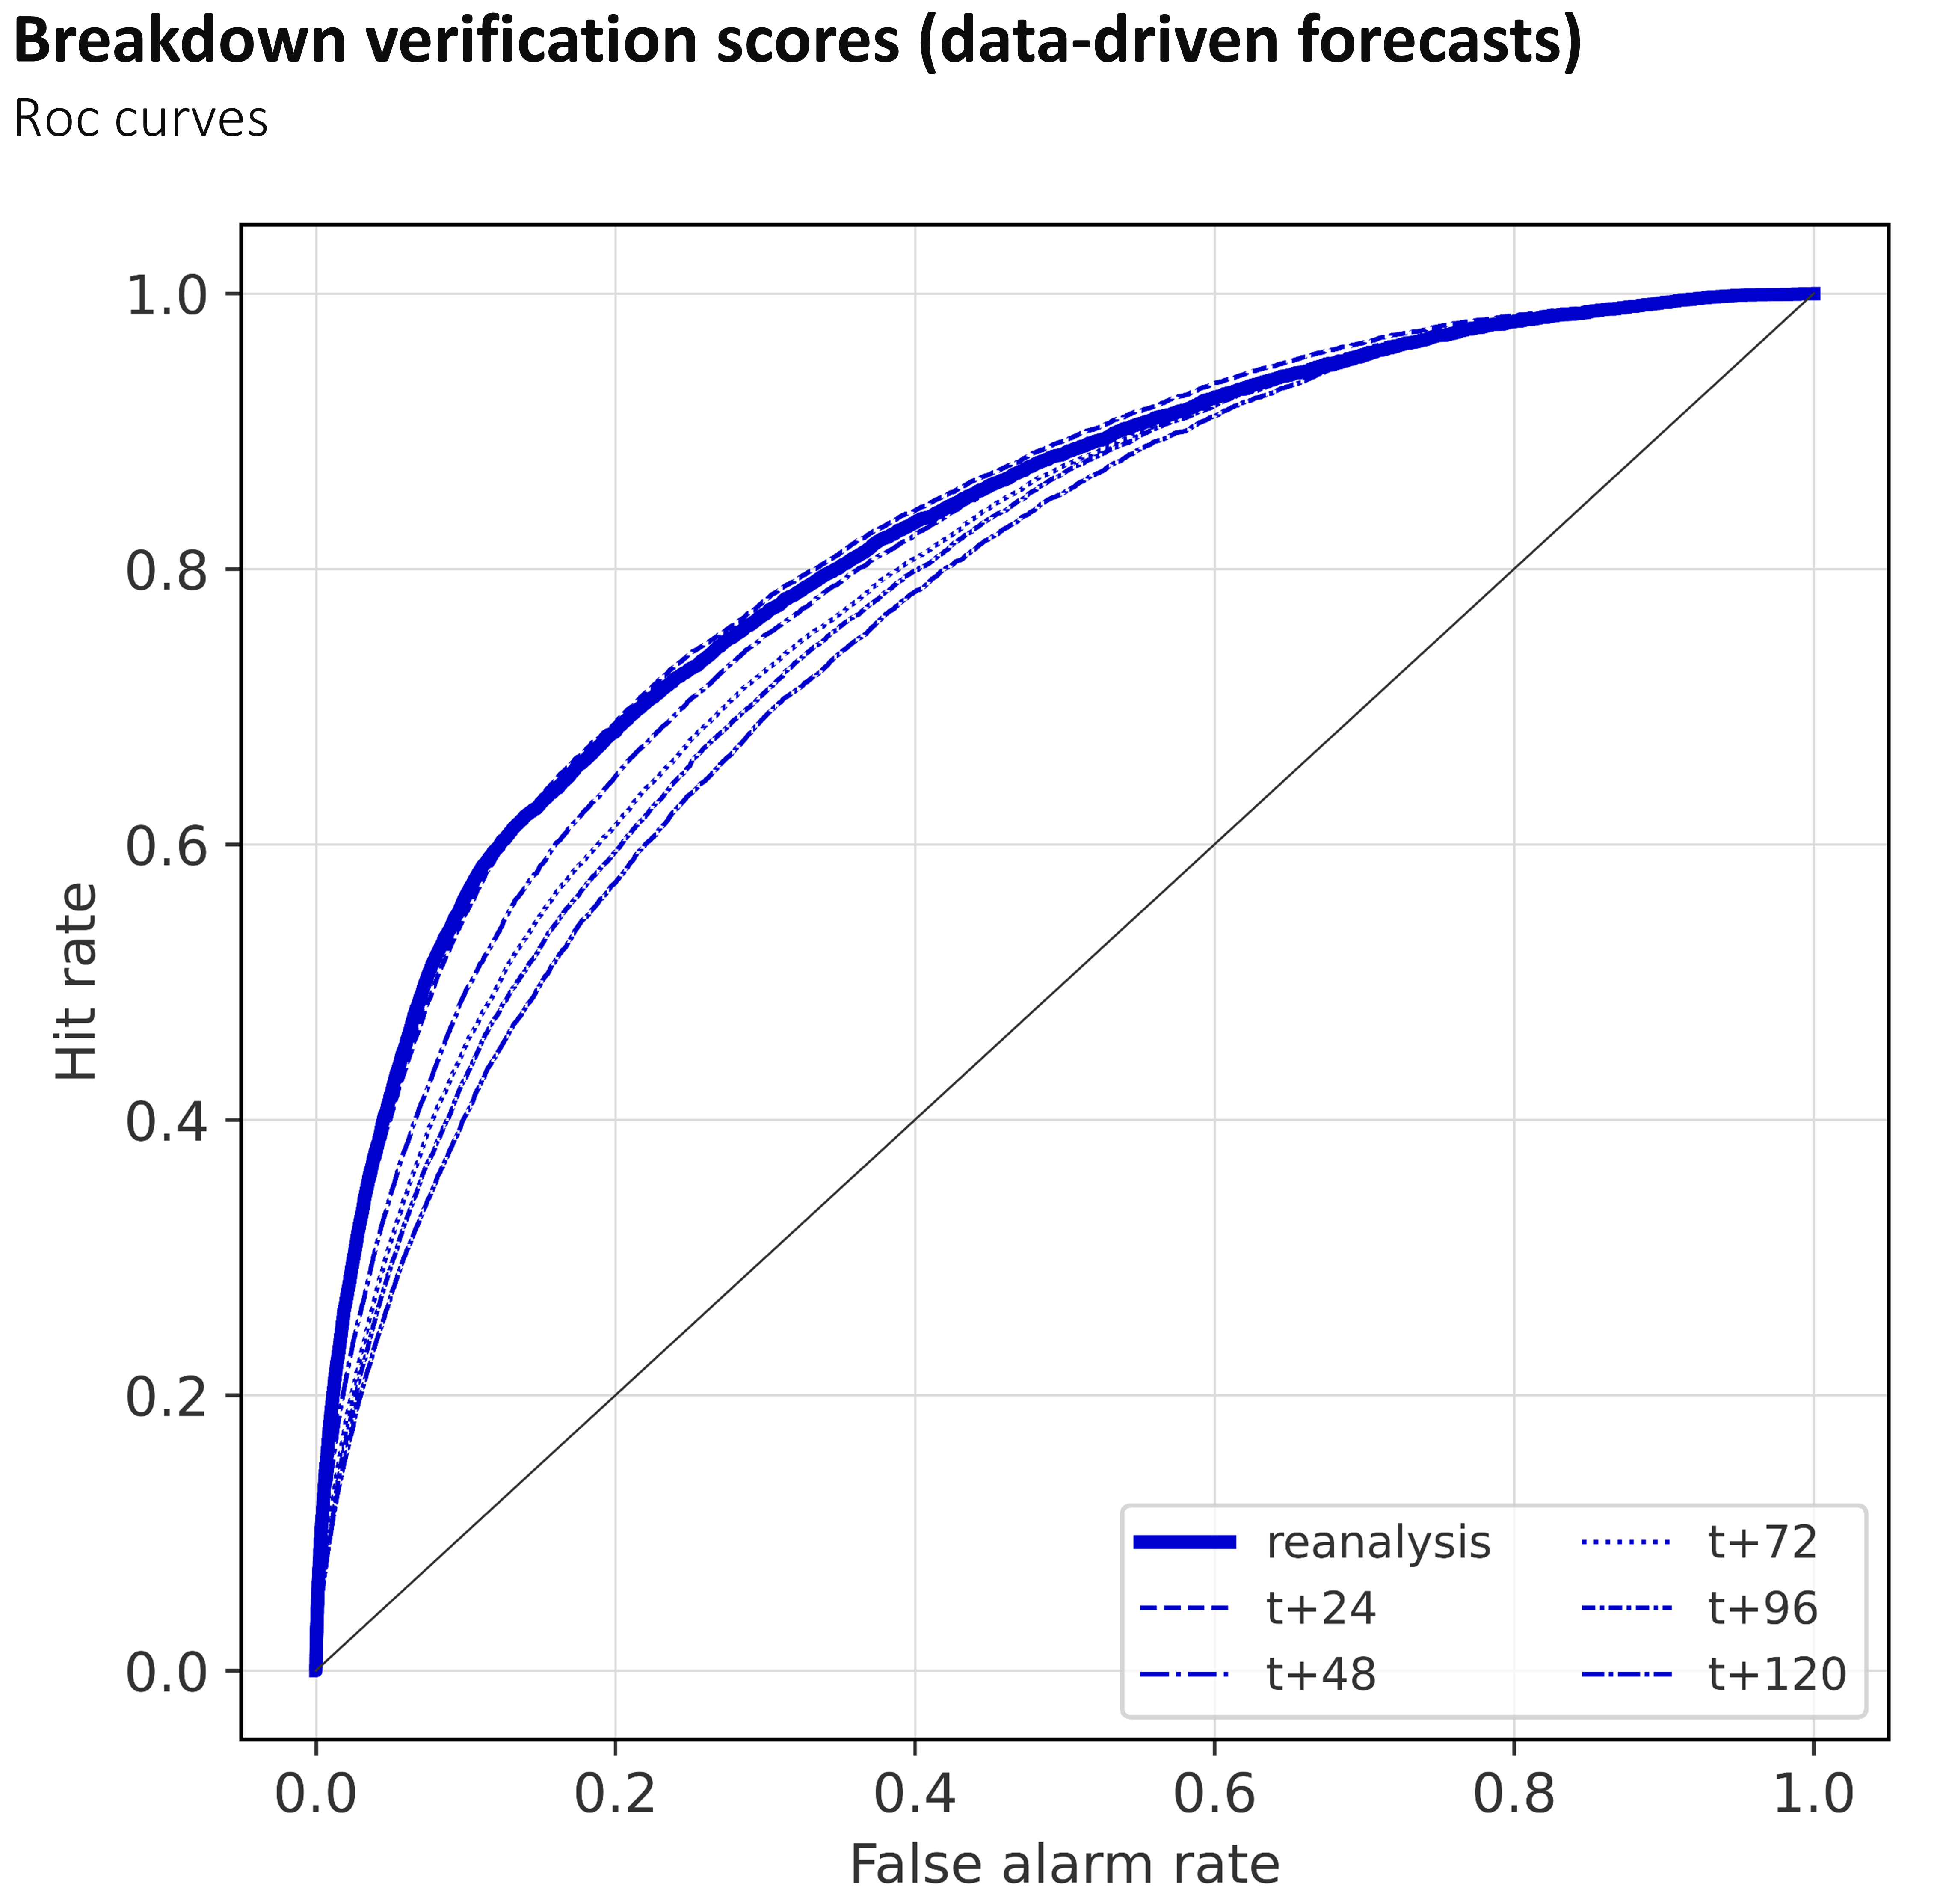
\includegraphics[width=\textwidth]{hydro_based_ff_verif_breakdown_scores_roc.png}
\caption{\textbf{Breakdown verification scores for data-driven, hydro-meteorological forecasts - ROC curves} Panels (a) to (f) show the ROC curves, respectively, for the short-range forecasts (i.e., reanalysis), for the long range forecasts at t+24 (day 1), t+48 (day 2), t+72 (day 3), t+96 (day 4), and t+120 (day 5).}
\label{fig:hydro_based_ff_verif_breakdown_scores_roc}
\end{figure}

From the reliability diagrams (Figure \ref{fig:hydro_based_ff_verif_breakdown_scores_rel_diag}) it is possible to understand better why the frequency bias increases significantly with the lead time \ref{fig:hydro_based_ff_verif_overall_scores}b. The reliability diagrams for day 0 (\ref{fig:hydro_based_ff_verif_breakdown_scores_rel_diag}a) and for day 1 (\ref{fig:hydro_based_ff_verif_breakdown_scores_rel_diag}b) are very similar. However, day 0 reliability shows a wider range of probabilities (up to \sim 15\%) with predicted probabilities similar to those observed than day 1 (with probabilities with this similar behaviour only up to \sim 10\%). At day 2 forecasts, the range of well calibrated probabilities diminishes up to 5\%, and from day 3, the predictions show mostly overestimation of the observed frequencies from forecasts probabilities exceeding 1\%. It is worth noticing how, also in the case of the rainfall-based forecasts, also the data-driven forecasts do not show a reduction of the issued probabilities with increasing lead times. As discussed in relevant section, this is due to the fact that we are using a rainfall forecasts that post-processed a deterministic system.

\begin{figure}[htbp]
\centering
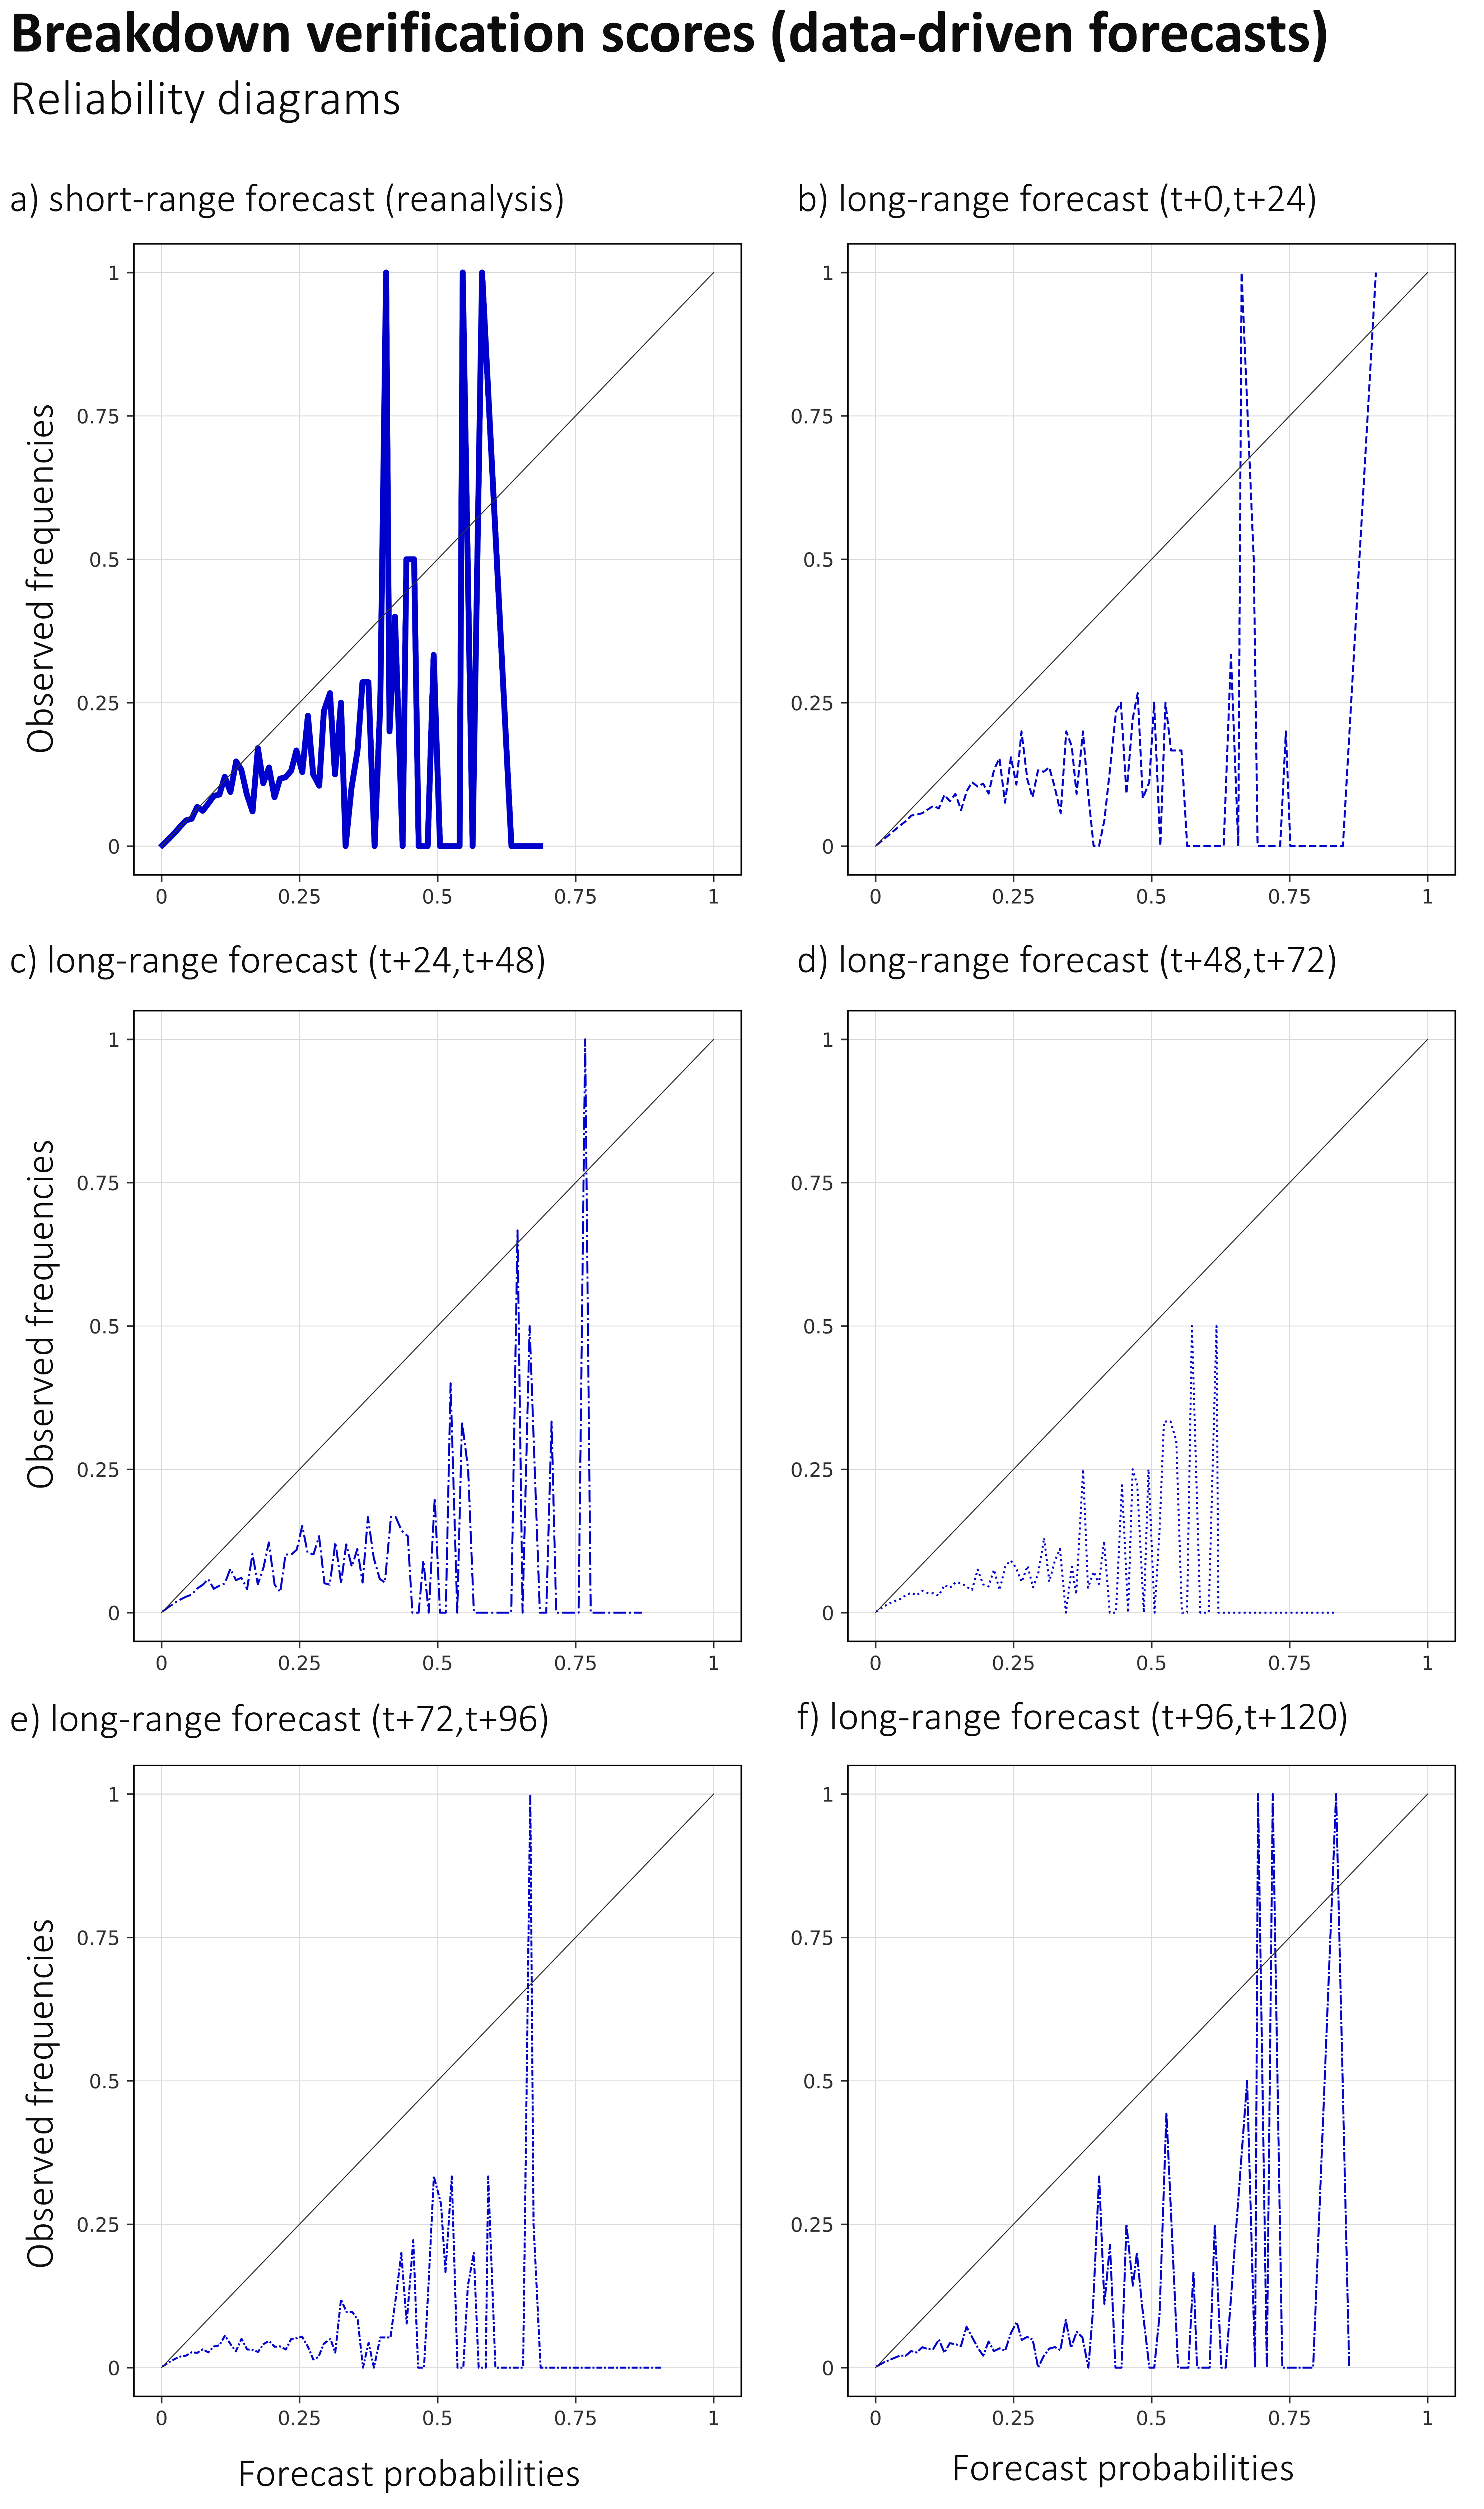
\includegraphics[width=\textwidth]{hydro_based_ff_verif_breakdown_scores_rel_diag.png}
\caption{\textbf{Breakdown verification scores for data-driven, hydro-meteorological forecasts - Reliability diagrams} Panels (a) to (f) show the reliability diagrams, respectively, for the short-range forecasts (i.e., reanalysis), for the long range forecasts at t+24 (day 1), t+48 (day 2), t+72 (day 3), t+96 (day 4), and t+120 (day 5).}
\label{fig:hydro_based_ff_verif_breakdown_scores_rel_diag}
\end{figure}


%%%%%%%%%%%%%%%%%%%%%%%%%%%%%%%%%%%%%%%%%%%%%%%%%%%%%%%%%%%%%%%%%%%%%%%
\subsection{Physical interpretation of the data-driven model behaviour}



%%%%%%%%%%%%%%%%%%%%%
\section{Discussions}
\label{data_driven_flash_floods_short_medium_range_discussions}

The results presented in the subsequent sections document the performance of both rainfall-based and data-driven hydro-meteorological forecasts. Section \ref{verif_rainfall_based_fc} shows the baseline verification results for the prediction of areas at risk of flash floods based using only ERA5-ecPoint short- and long-range rainfall predictions. Section \ref{verif_data_driven_short_fc} shows that the data-driven approach combining hydro-meteorological parameters yields statistically significant improvements in prediction skill, with particularly notable gains in discrimination ability as seen in the provided ROC curves. Section \ref{verif_data_driven_long_fc} shows that the predictive skill of the data-driven forecasts extends to day 5 with my better discrimination ability than its only rainfall-based counterpart. Section \ref{verif_case_study} shows a selection of flash flood events to illustrate the approaches' capacity to identify areas at risk of flash floods (in the US and around the world). Hence, the findings detailed in this chapter contribute to understanding how effectively current technologies can support flash flood warning systems.



%%%%%%%%%%%%%%%%%%%%%
\section{Conclusions}
\label{data_driven_flash_floods_short_medium_range_conclusions}

